\chapter{Supplemental Material for Chapter \ref{chap:chapter 2}}

%%%%%%%%%%%%%%%%%%%%%%%%%%%%%%%%%%%%%%%%%%%%%%%%%%%%%%%%%%%%%%%%%%%%%%%%%%%%%%%%
\section{Supplementary Figures}
%%%%%%%%%%%%%%%%%%%%%%%%%%%%%%%%%%%%%%%%%%%%%%%%%%%%%%%%%%%%%%%%%%%%%%%%%%%%%%%%

\begin{figure}[p]
    \centering
    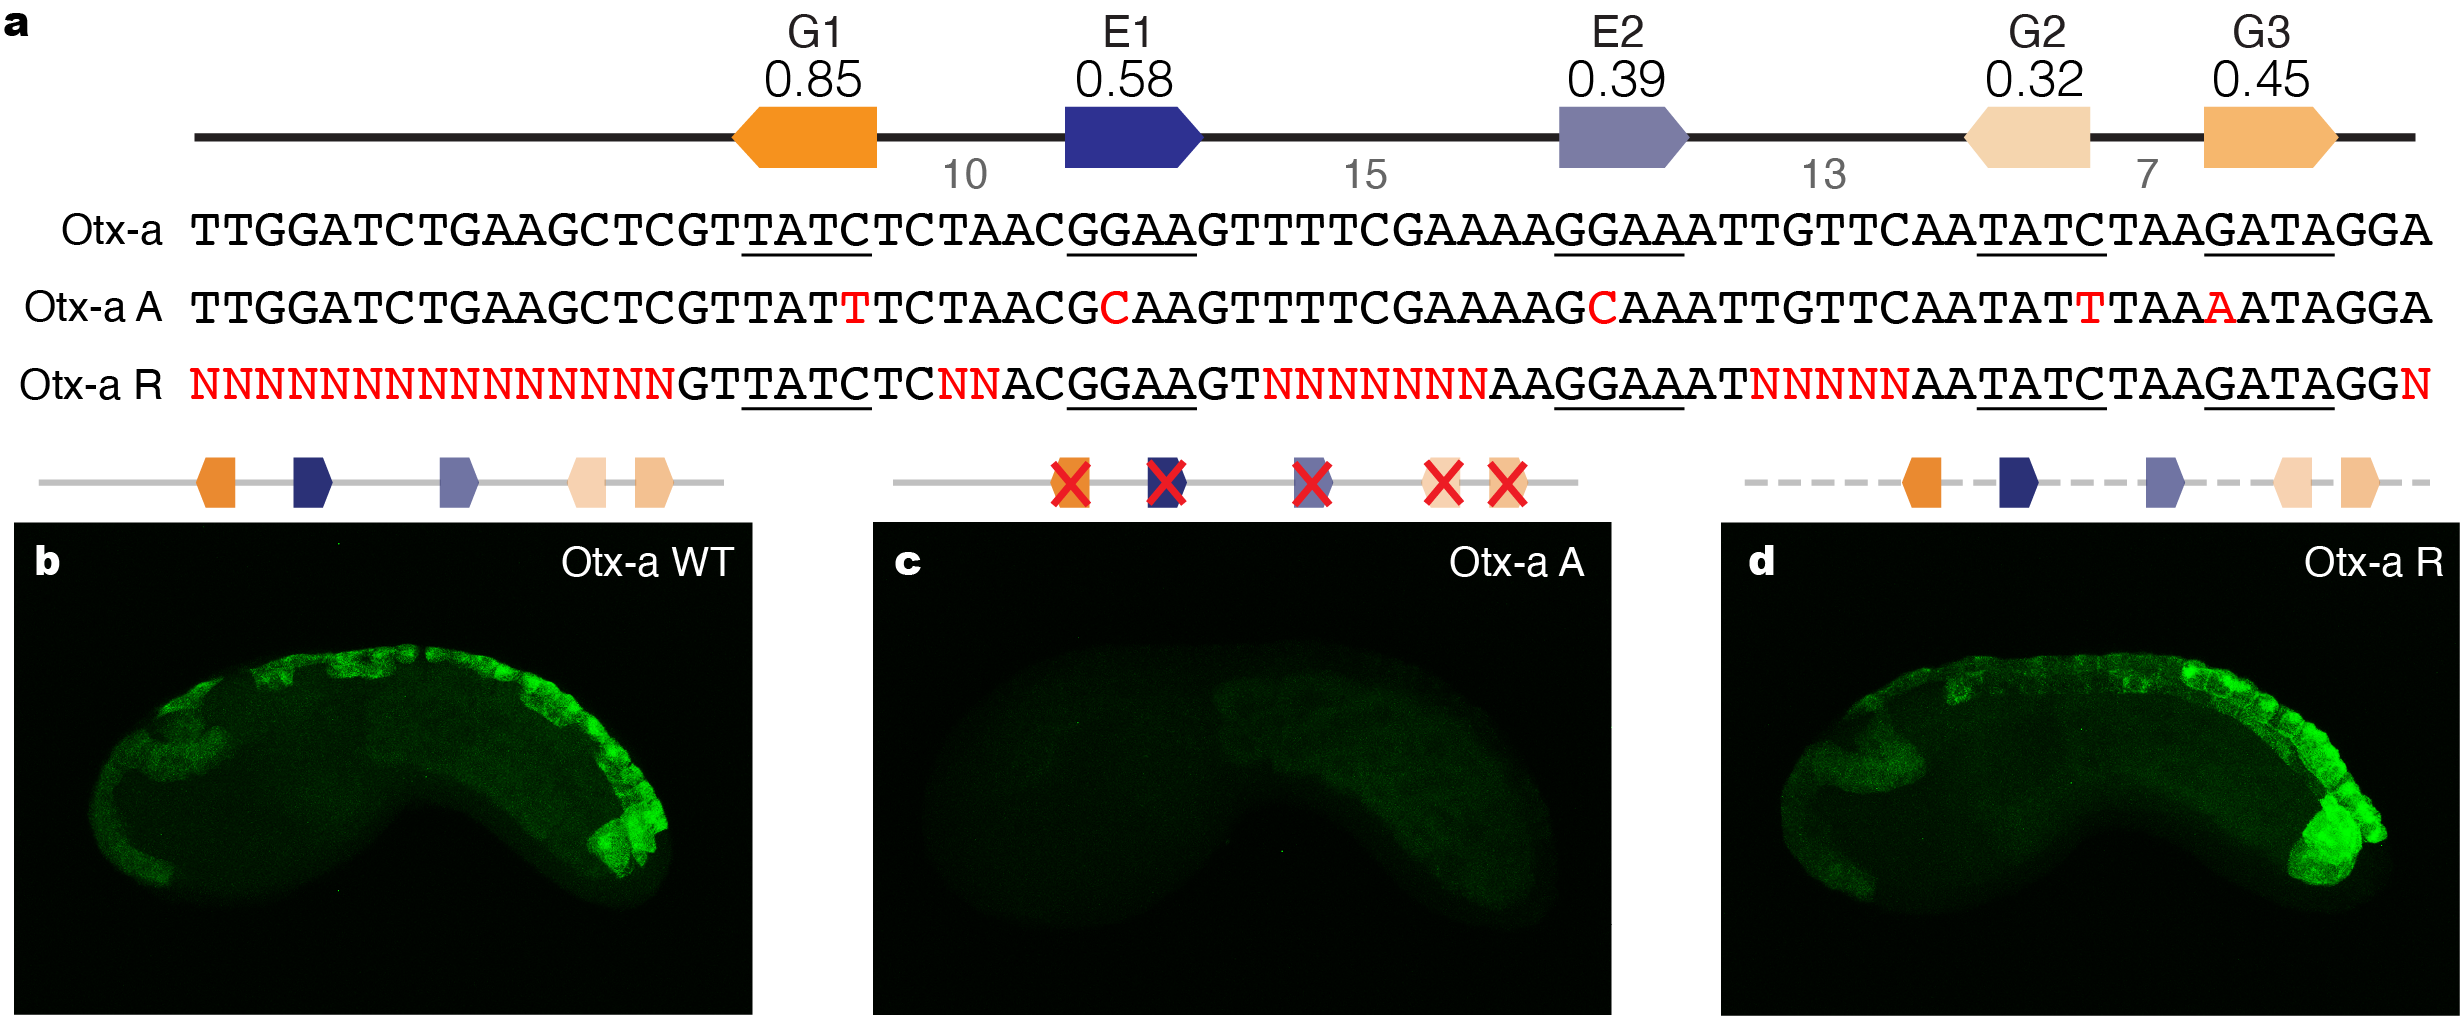
\includegraphics[width=0.85\textwidth]{2_figures-and-files/SuppFig1.png}
    \caption[Defining the necessary and sufficient TFBS for Otx-a enhancer activity.]{\textbf{Defining the necessary and sufficient TFBS for Otx-a enhancer activity.} \textbf{a)} Otx-a contains three GATA and two ETS sites. The GATA and ETS core sequences that hydrogen bond to the TF are underlined, GATA and GGAW respectively. The relative affinity is labelled above each site and is defined by the nucleotides flanking the cores. Spacing between the sites is shown in gray numbers. Otx-a Ablated (Otx-a A) contains single point mutations within the core of each binding site that ablate binding of the TF. The Otx-a Randomized (Otx-a R) library contains 5 million unique sequences where the GATA and ETS sites are fixed, but the linker sequences are randomized (denoted with Ns which represent equal chance of A, T, G or C). \textbf{e)} Otx-a WT enhancer activates expression in the a6.5 and b6.5 lineages. \textbf{f)} Otx-a A does not activate expression. \textbf{g)} Otx-a R activates neural expression that is indistinguishable from Otx-a WT despite the randomization of linker sequences.}
    \label{fig:2 supplementary_1}
\end{figure}

\begin{figure}[p]
    \centering
    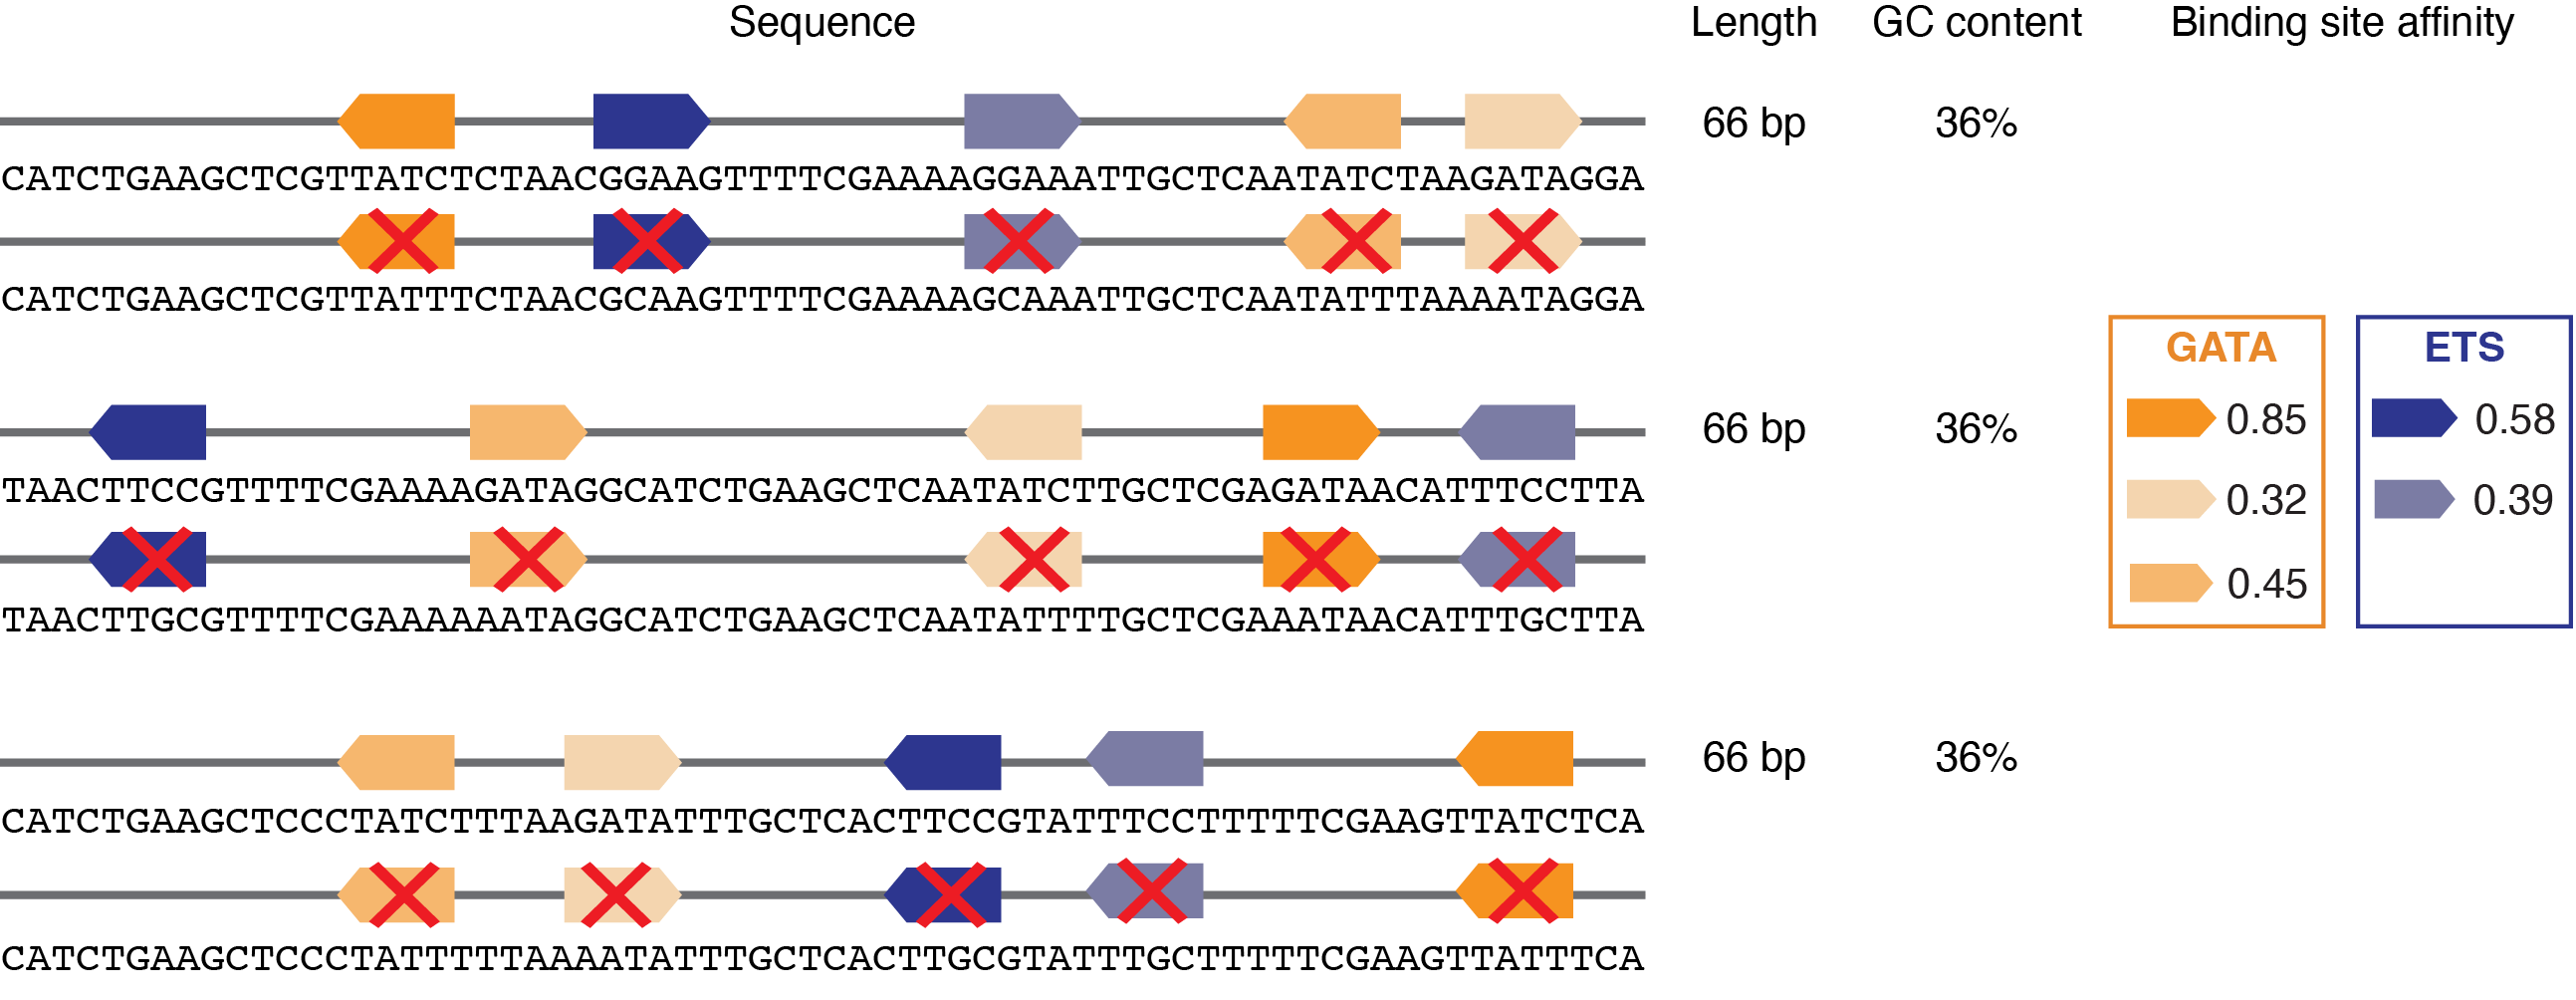
\includegraphics[width=0.75\textwidth]{2_figures-and-files/SuppFig2.png}
    \caption[Examples of Otx-a scrambled library variants and their ablated counterparts.]{\textbf{Examples of Otx-a scrambled library variants and their ablated counterparts.} Each element has the same sequence content, GC content, and binding sites. The only difference between the members is the order, orientation, spacing and placement of the different affinity binding sites.}
    \label{fig:2 supplementary_2}
\end{figure}

\begin{figure}[p]
    \centering
    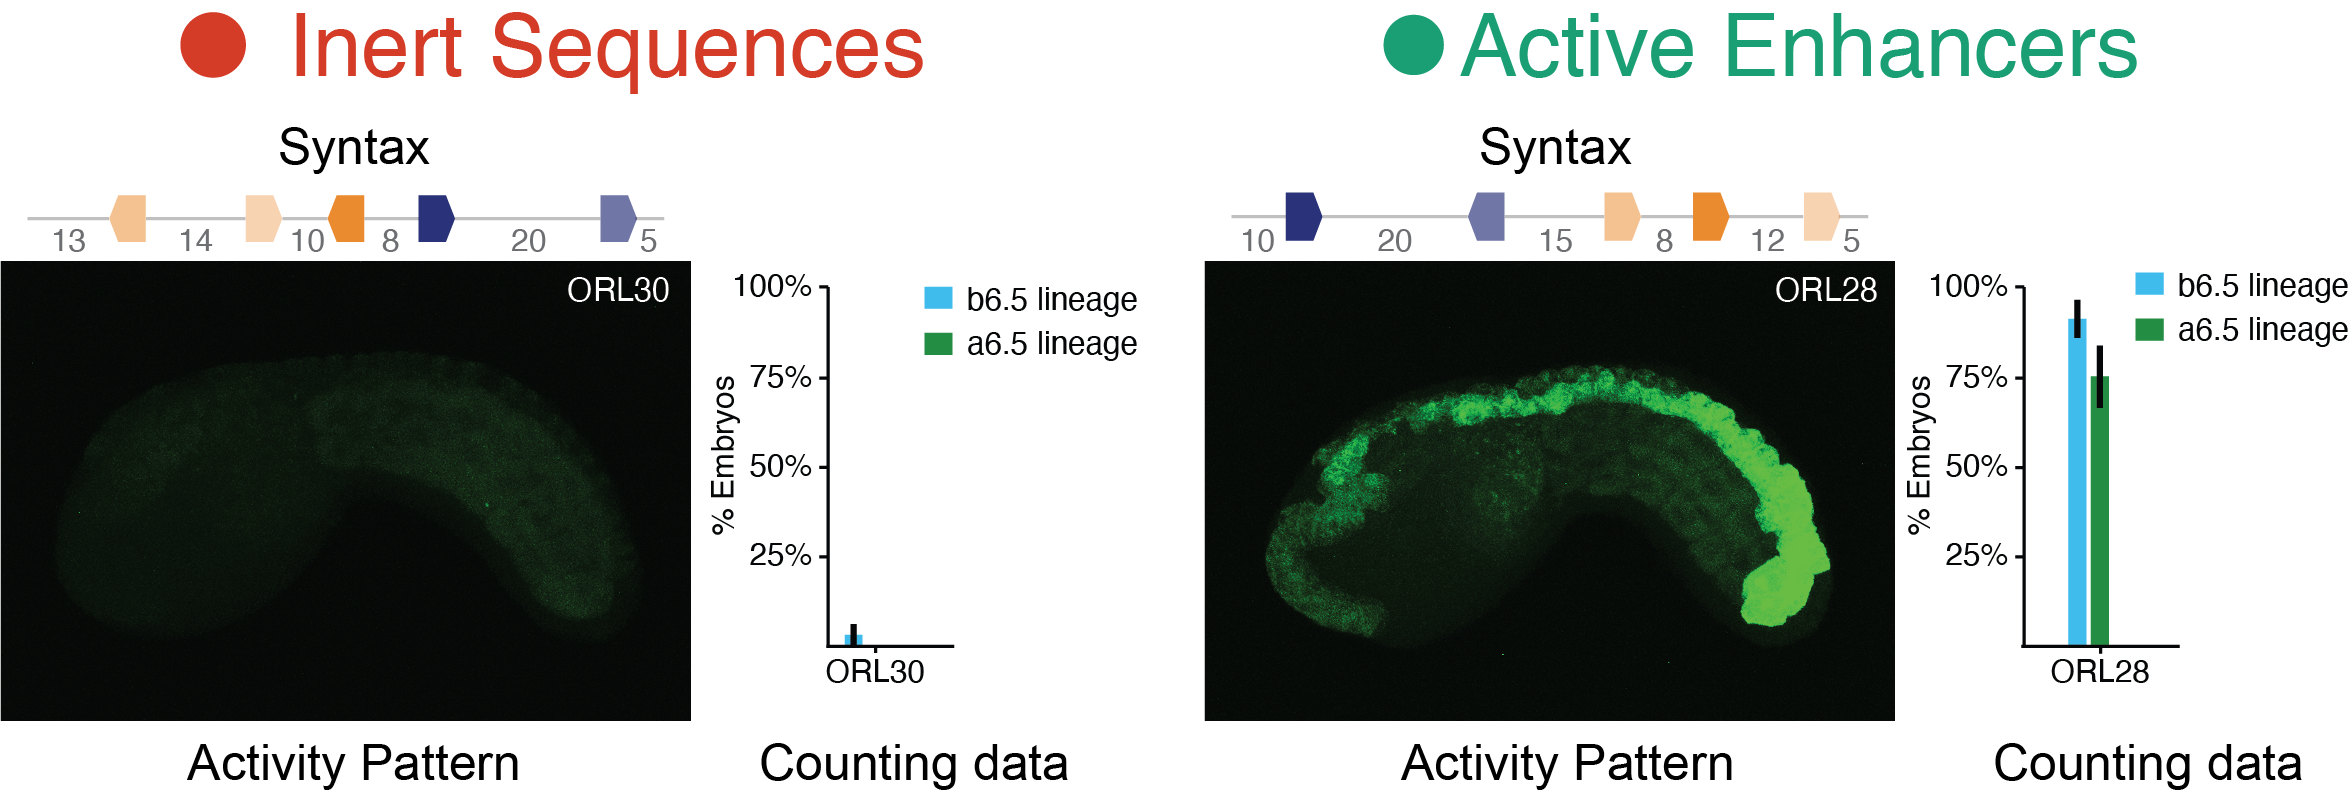
\includegraphics[width=0.85\textwidth]{2_figures-and-files/SuppFig3.png}
    \caption[Examples of microscope validated classification labels of library elements.]{\textbf{Examples of microscope validated classification labels of library elements.} 23 OSL elements were randomly selected for validation with fluorescence microscopy and classified as Inert Sequences or Active Enhancers based on counting data (\textbf{Figure~\ref{fig:2 Figure 1}g}). \textbf{Left,} example syntax with no expression classified as Inert Sequence. \textbf{Right,} example syntax with Otx-a WT like expression classified as Active Enhancer. Counting data for a6.5 and b6.5 lineage activity in 50 embryos is shown.}
    \label{fig:2 supplementary_3}
\end{figure}

\begin{figure}[p]
    \centering
    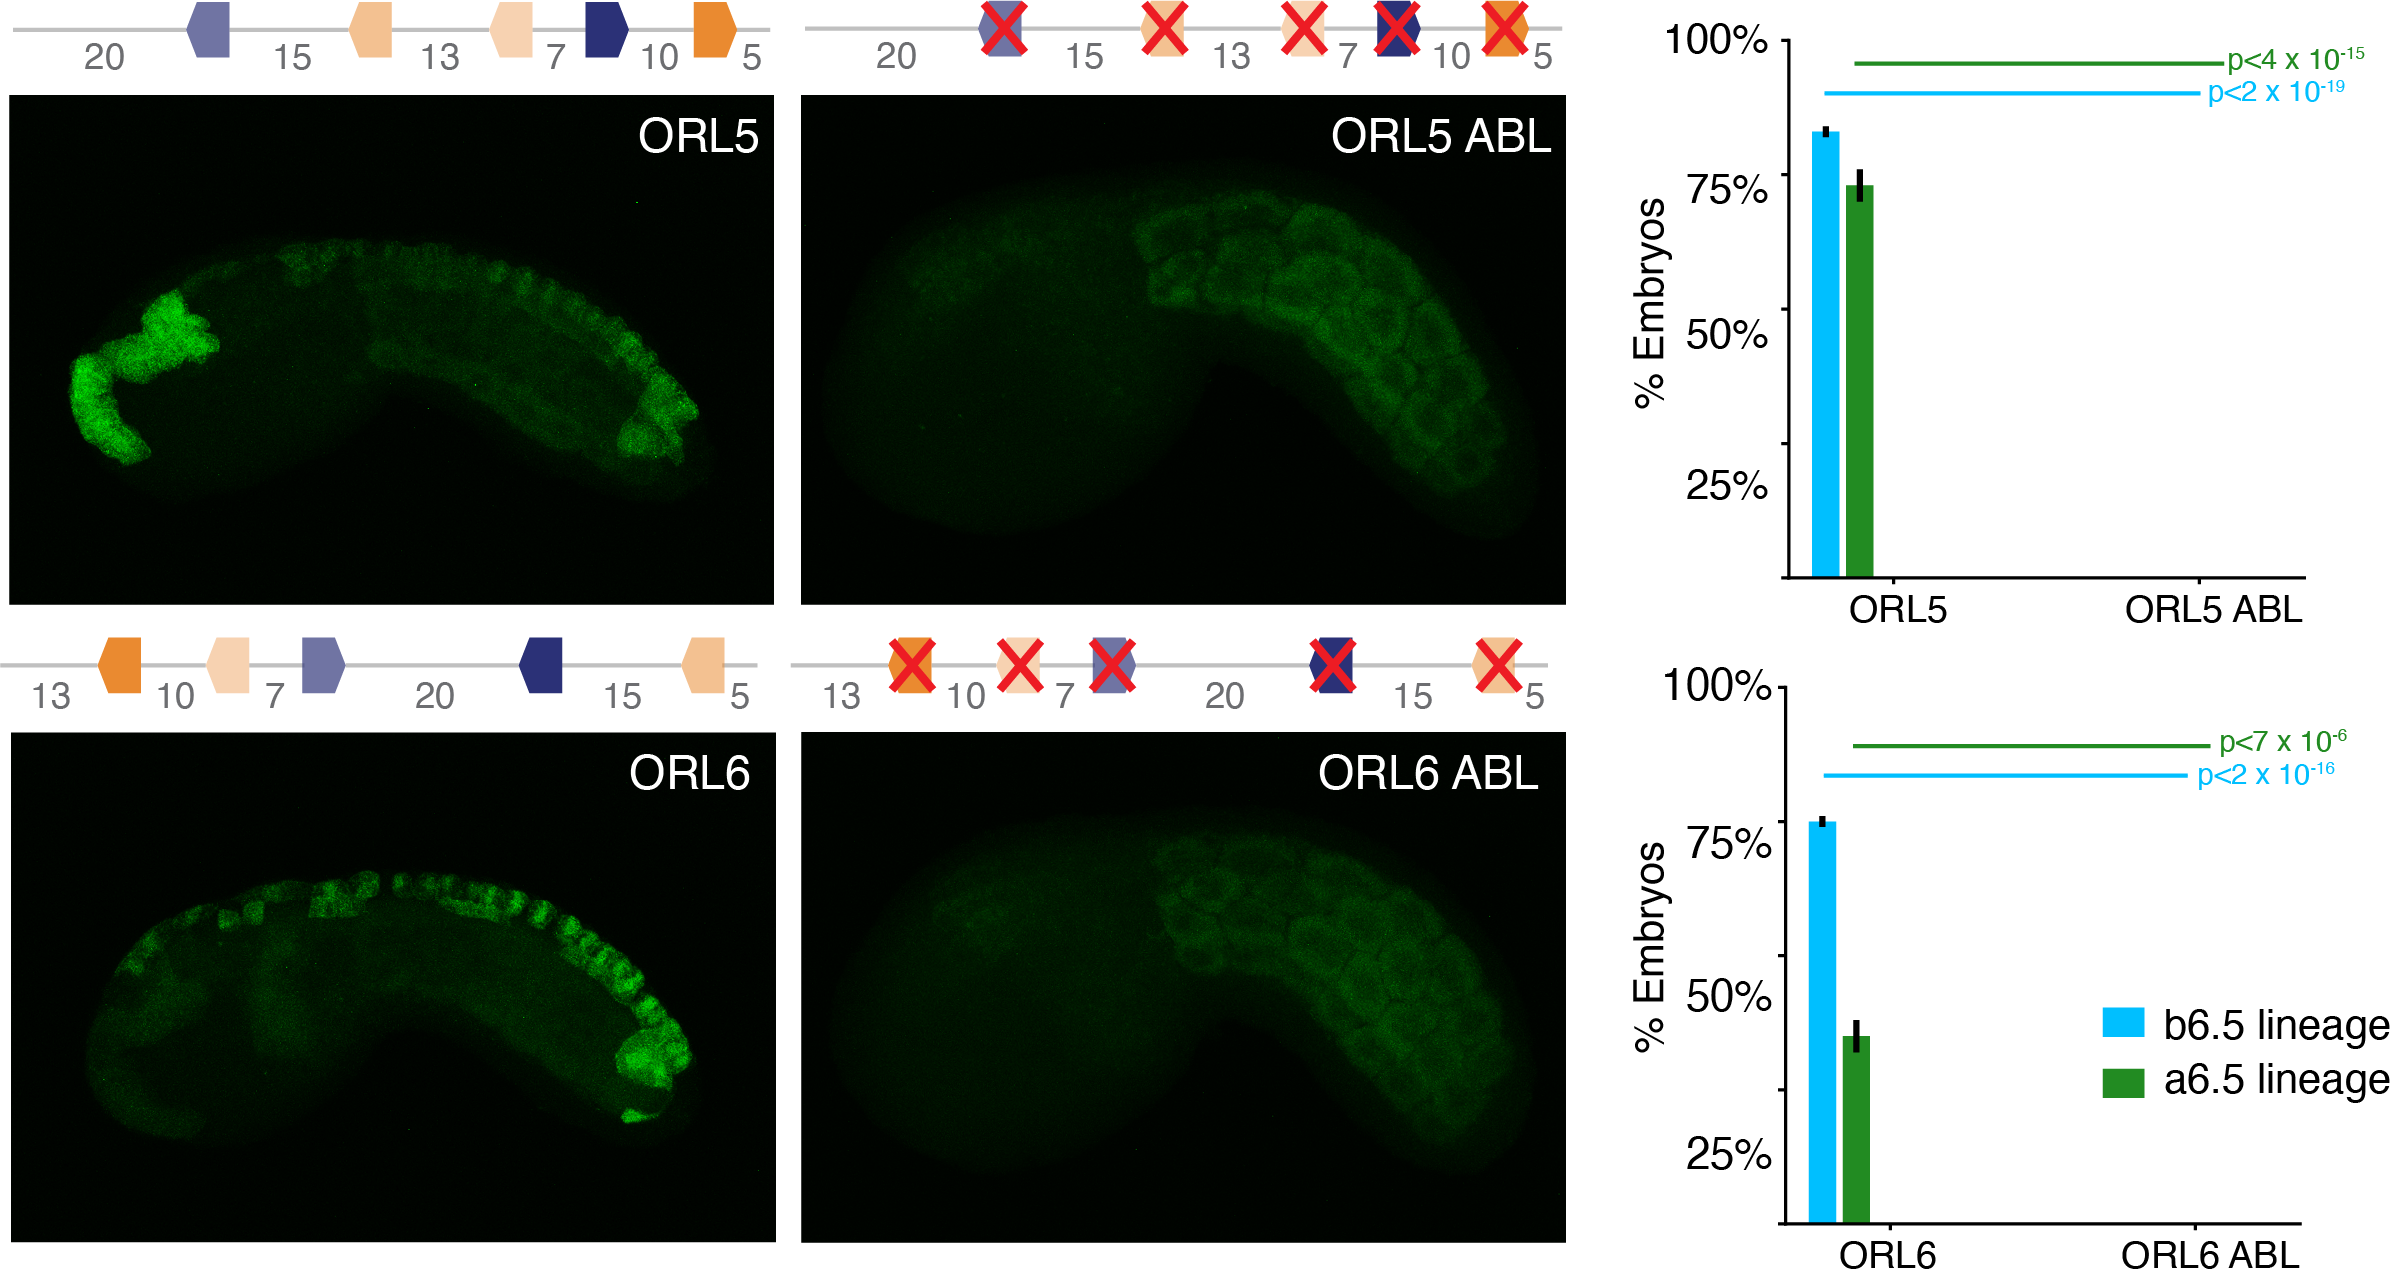
\includegraphics[width=0.9\textwidth]{2_figures-and-files/SuppFig4.png}
    \caption[GATA and ETS are required for neural expression of Otx-a scrambled elements.]{\textbf{GATA and ETS are required for neural expression of Otx-a scrambled elements.} \textbf{a)} OSL5 activates expression in the a6.5 and b6.5 lineages. \textbf{b)} OSL5 ABL construct in which all the GATA and ETS sites are ablated by point mutations (indicated with red Xs) activates no expression. \textbf{c)} Counting for OSL5 and OSL5 ABL shows \% of embryos with expression in the a6.5 and b6.5 lineages. 50 embryos counted in each replicate. \% embryos with expression is significantly different between OSL5 and OSL5 ABL (p < 4e-15 Fisher’s exact test, 2 replicates of 50 embryos each). \textbf{d)} OSL6 enhancer drives expression in the a6.5 and b6.5 lineage neural tissues. \textbf{e)} OSL6 ABL activates no expression. \textbf{f)} Counting data for OSL6 and OSL6 ABL shows \% of embryos with expression in the a6.5 and b6.5 lineages. 50 embryos counted in each replicate. \% embryos with expression is significantly different between OSL6 and OSL6 ABL (p < 4e-15 Fisher’s exact test, 2 replicates of 50 embryos each).}
    \label{fig:2 supplementary_4}
\end{figure}

\begin{figure}[p]
    \centering
    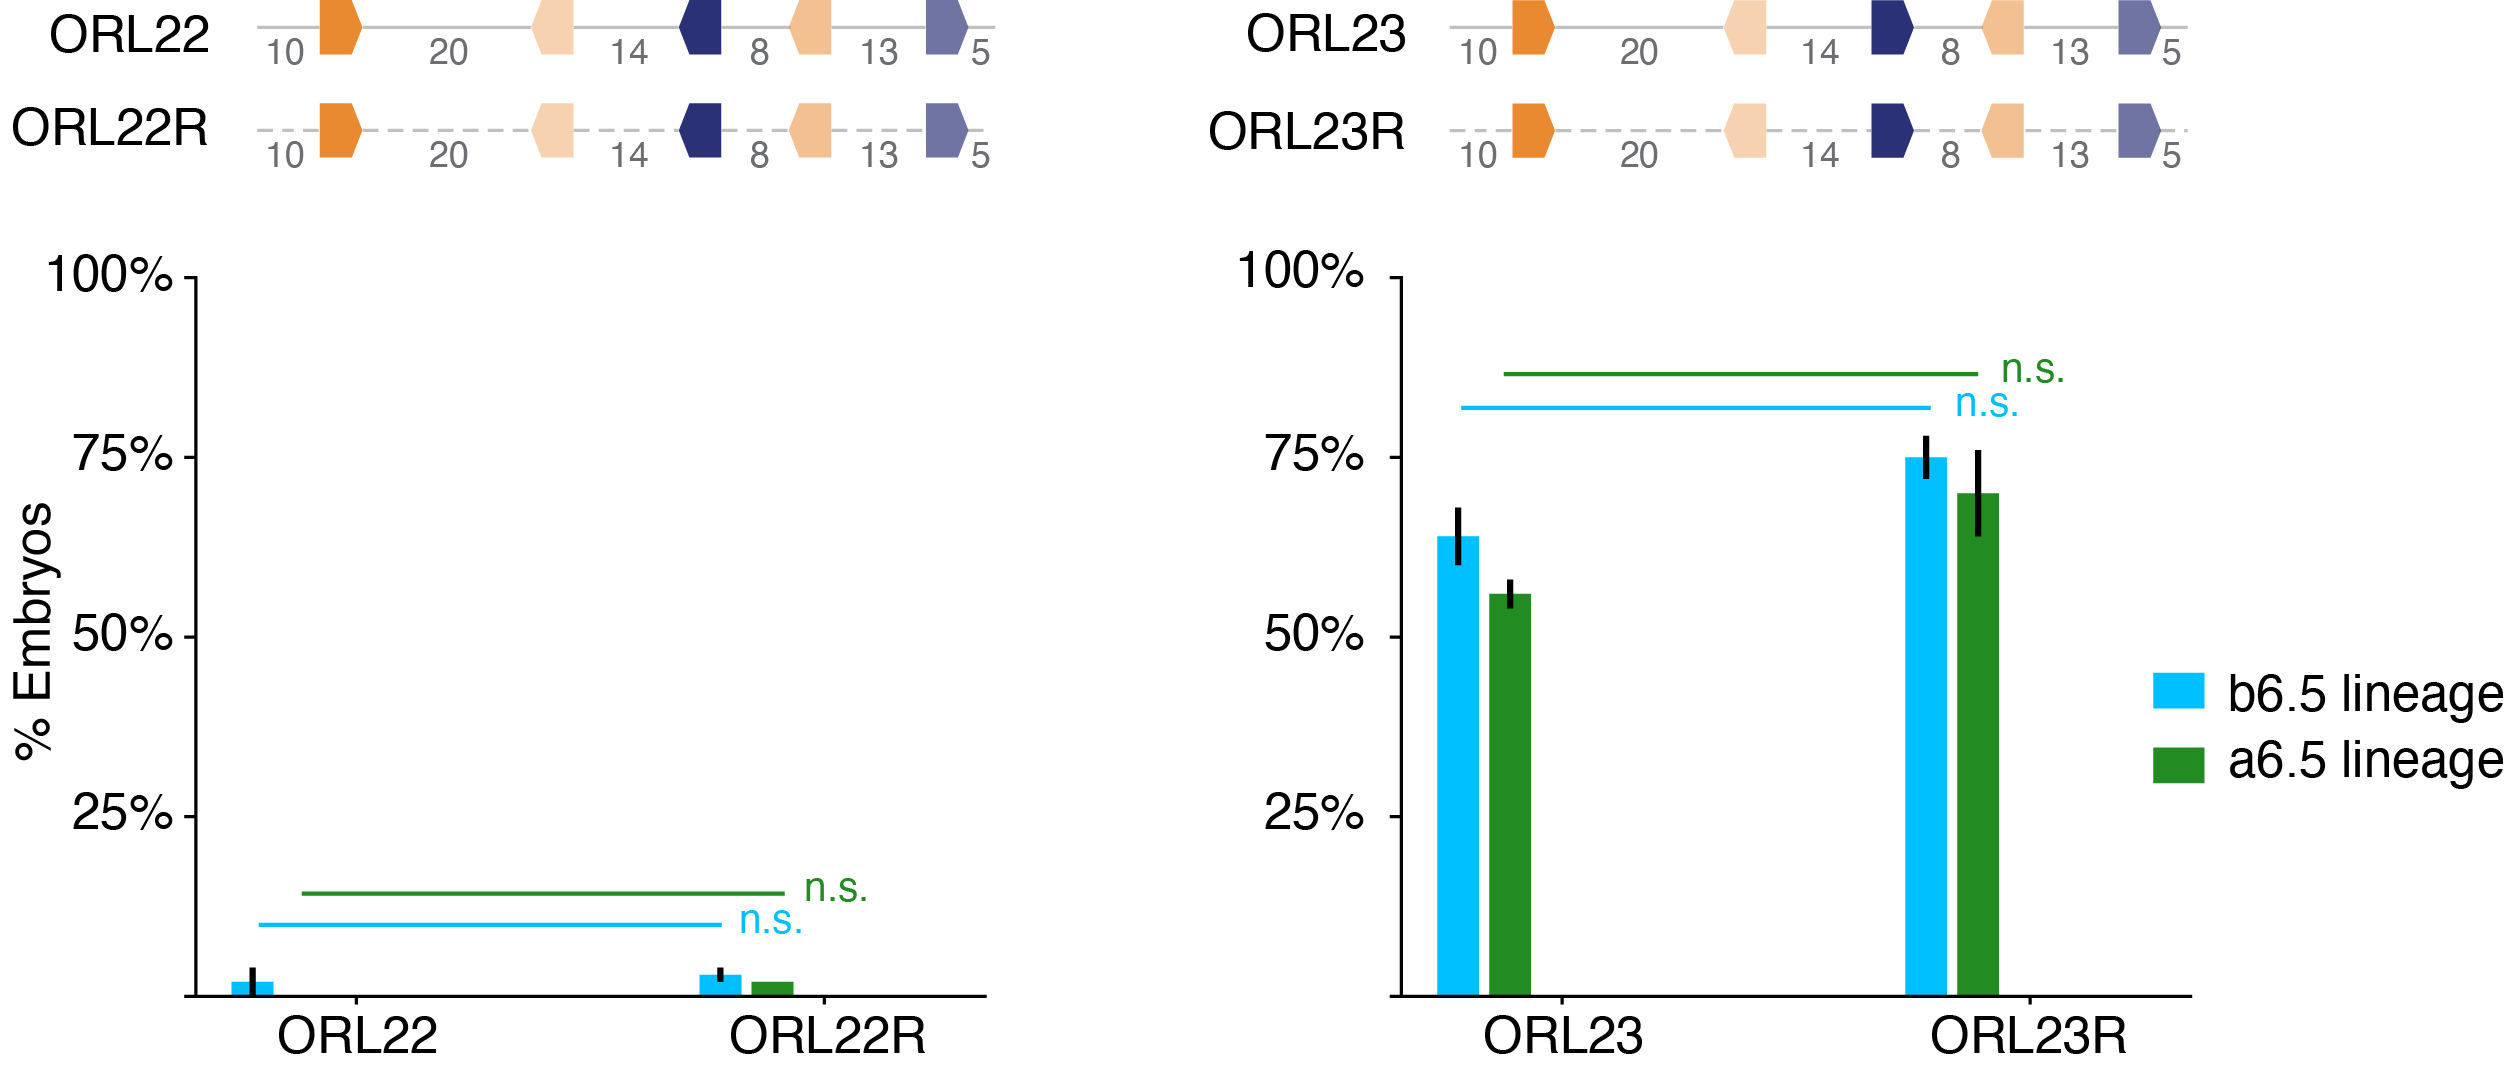
\includegraphics[width=0.85\textwidth]{2_figures-and-files/SuppFig5.png}
    \caption[Organization of binding sites matters for encoding active enhancers.]{\textbf{Organization of binding sites matters for encoding active enhancers.} \textbf{a)} In the randomized construct OSL22R, all bases of the linker sequences are replaced with N nucleotides which represent an equal chance of A, T, G or C. More than 3 million unique sequences in the OSL22R library. OSL22 and OSL22R have no significant difference in percent embryos with expression in either a6.5 or b6.5 lineages (Fisher’s exact test, two replicates of 50 embryos each). \textbf{b)} OSL23 is an element activating expression in a6.5 and b6.5 neural tissues. OSL23R with randomized linker sequences, comprising over 3 million unique sequences, is not significantly different from OSL23 in change in percent embryos with expression (Fisher’s exact test, two replicates of 50 embryos each).}
    \label{fig:2 supplementary_5}
\end{figure}

\begin{figure}[p]
    \centering
    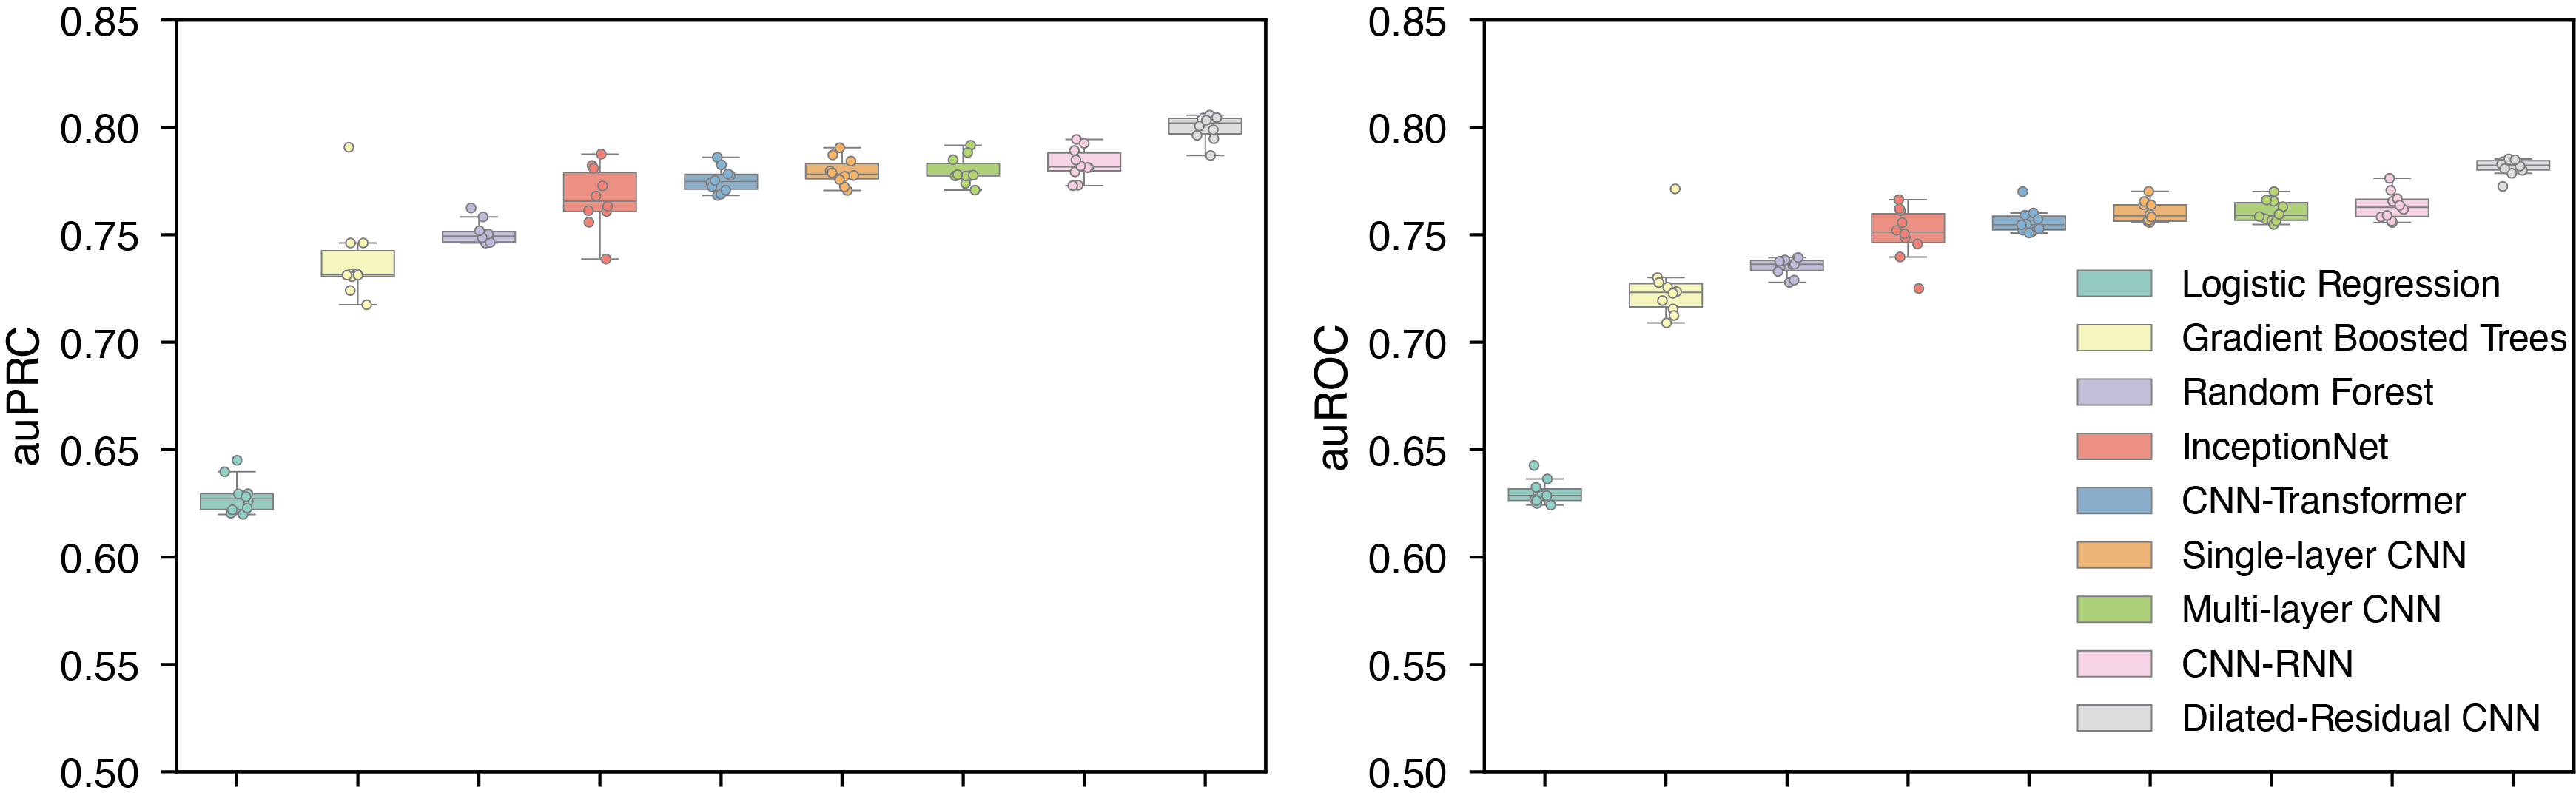
\includegraphics[width=0.85\textwidth]{2_figures-and-files/SuppFig6.png}
    \caption[10-fold cross validation performance of syntax models.]{\textbf{10-fold cross validation performance of syntax models.} 10-fold cross validation area under the precision-recall curve (auPRC, left) and area under the receiver operating characteristic curve (auROC, right) for several classes of machine learning model. The box plots show distributions for each performance metric and each point represents the performance on an individual fold of the data. The boxes show medians along with low and high quartiles. Whiskers extend to the furthest datapoint within 1.5-times the interquartile range. More extreme points are marked as outliers.}
    \label{fig:2 supplementary_6}
\end{figure}

\begin{figure}[p]
    \centering
    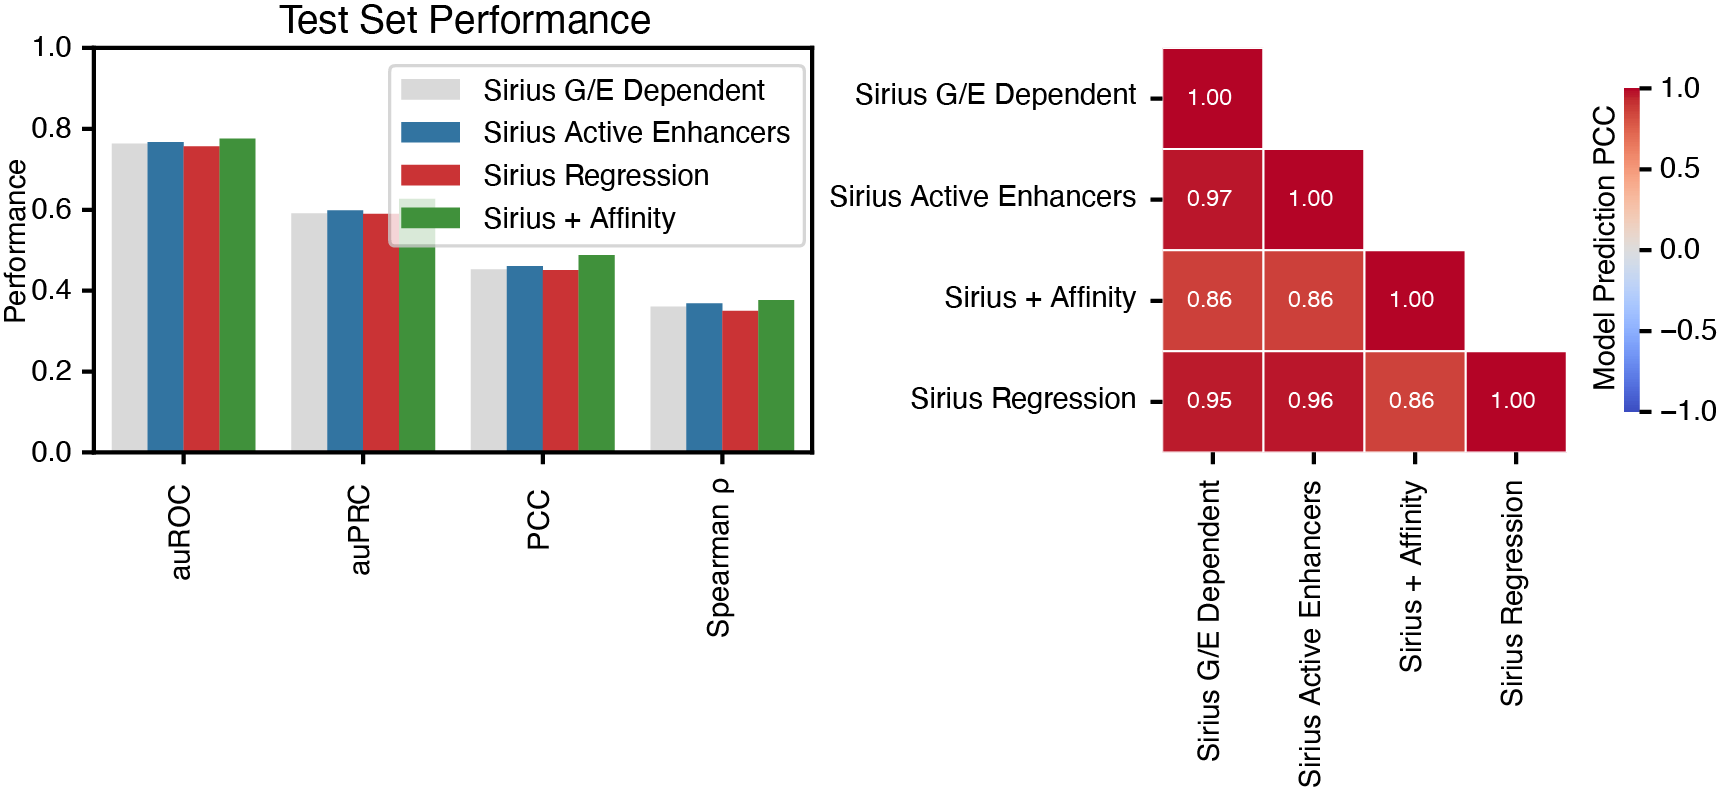
\includegraphics[width=0.85\textwidth]{2_figures-and-files/SuppFig7.png}
    \caption[Sirius predictions are robust to different training strategies.]{\textbf{Sirius predictions are robust to different training strategies.} \textbf{a)} Comparison of different training strategies across four performance metrics: area under the receiver operator characteristic curve (auROC), area under the precision-recall curve (auPRC), Pearson correlation coefficient (PCC), and Spearman’s $rho$. \textbf{b)} Heatmap shows pairwise PCC of test-set predictions for each model type (see Methods). Briefly, Sirius G/E Dependent refers to Sirius models trained on active enhancers driven by GATA and ETS sites (N=52,139). Sirius Active Enhancers refers to Sirius models trained on all active enhancers (N=80,965). Sirius Regression refers to models trained to predict the quantitative enhancer activity level using all detected sequences (N=393,554). Sirius + Affinity are trained on active enhancers driven by GATA and ETS sites, but use separate channels for each GATA affinity (G1, G2, and G3) and each ETS affinity (E1 and E2).}
    \label{fig:2 supplementary_7}
\end{figure}

\begin{figure}[p]
    \centering
    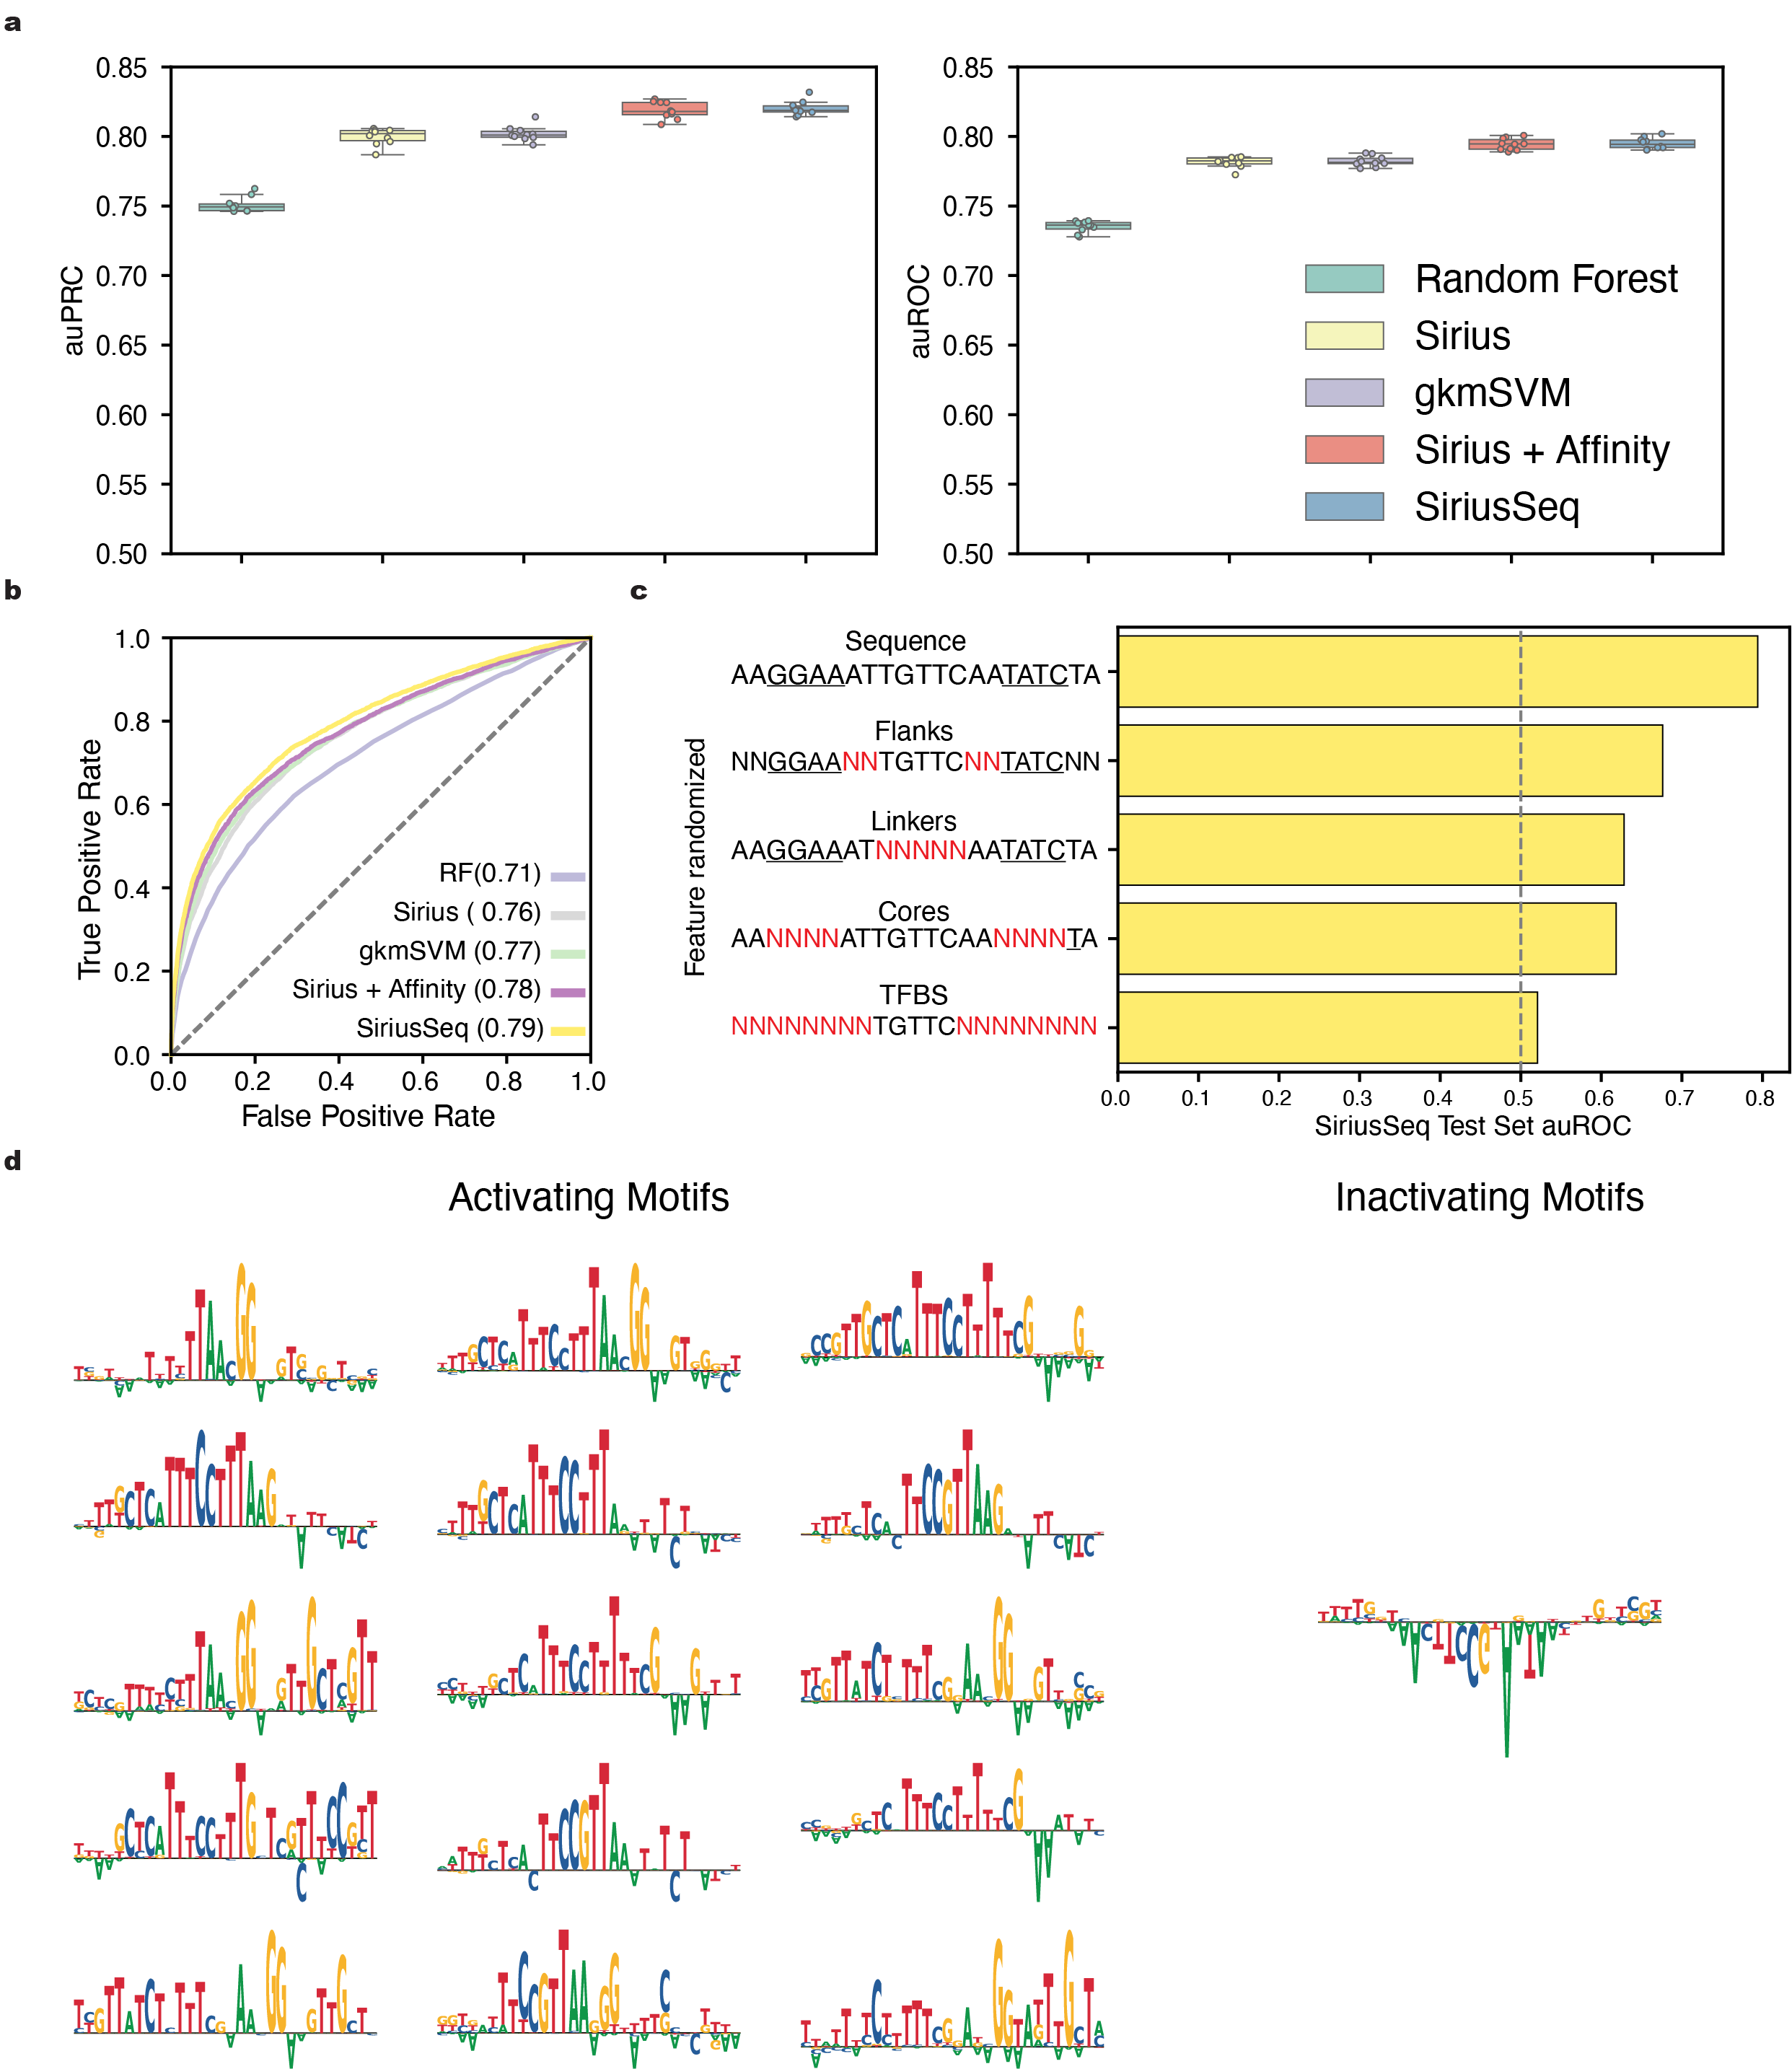
\includegraphics[width=0.85\textwidth]{2_figures-and-files/SuppFig8.png}
    \caption[Models trained on linear DNA sequence learn non-syntax features that marginally contribute to predictive performance.]{\textbf{Models trained on linear DNA sequence learn non-syntax features that marginally contribute to predictive performance.} \textbf{a)} 10-fold cross validation auPRC (left) and auROC (right) for several classes of machine learning model. The box plots show distributions for each performance metric and each point represents the performance on an individual fold of the data. The boxes show medians along with low and high quartiles. Whiskers extend to the furthest datapoint within 1.5-times the interquartile range. More extreme points are marked as outliers. \textbf{b)} Receiver operator characteristic curves for the same models as in \textbf{a)}. \textbf{c)} SiriusSeq held-out test set auROCs on sequences with the indicated randomized features. \textbf{d)} TF-MoDISco discovered motifs from SiriusSeq split into activating and inactivating motifs.}
    \label{fig:2 supplementary_8}
\end{figure}

\begin{figure}[p]
    \centering
    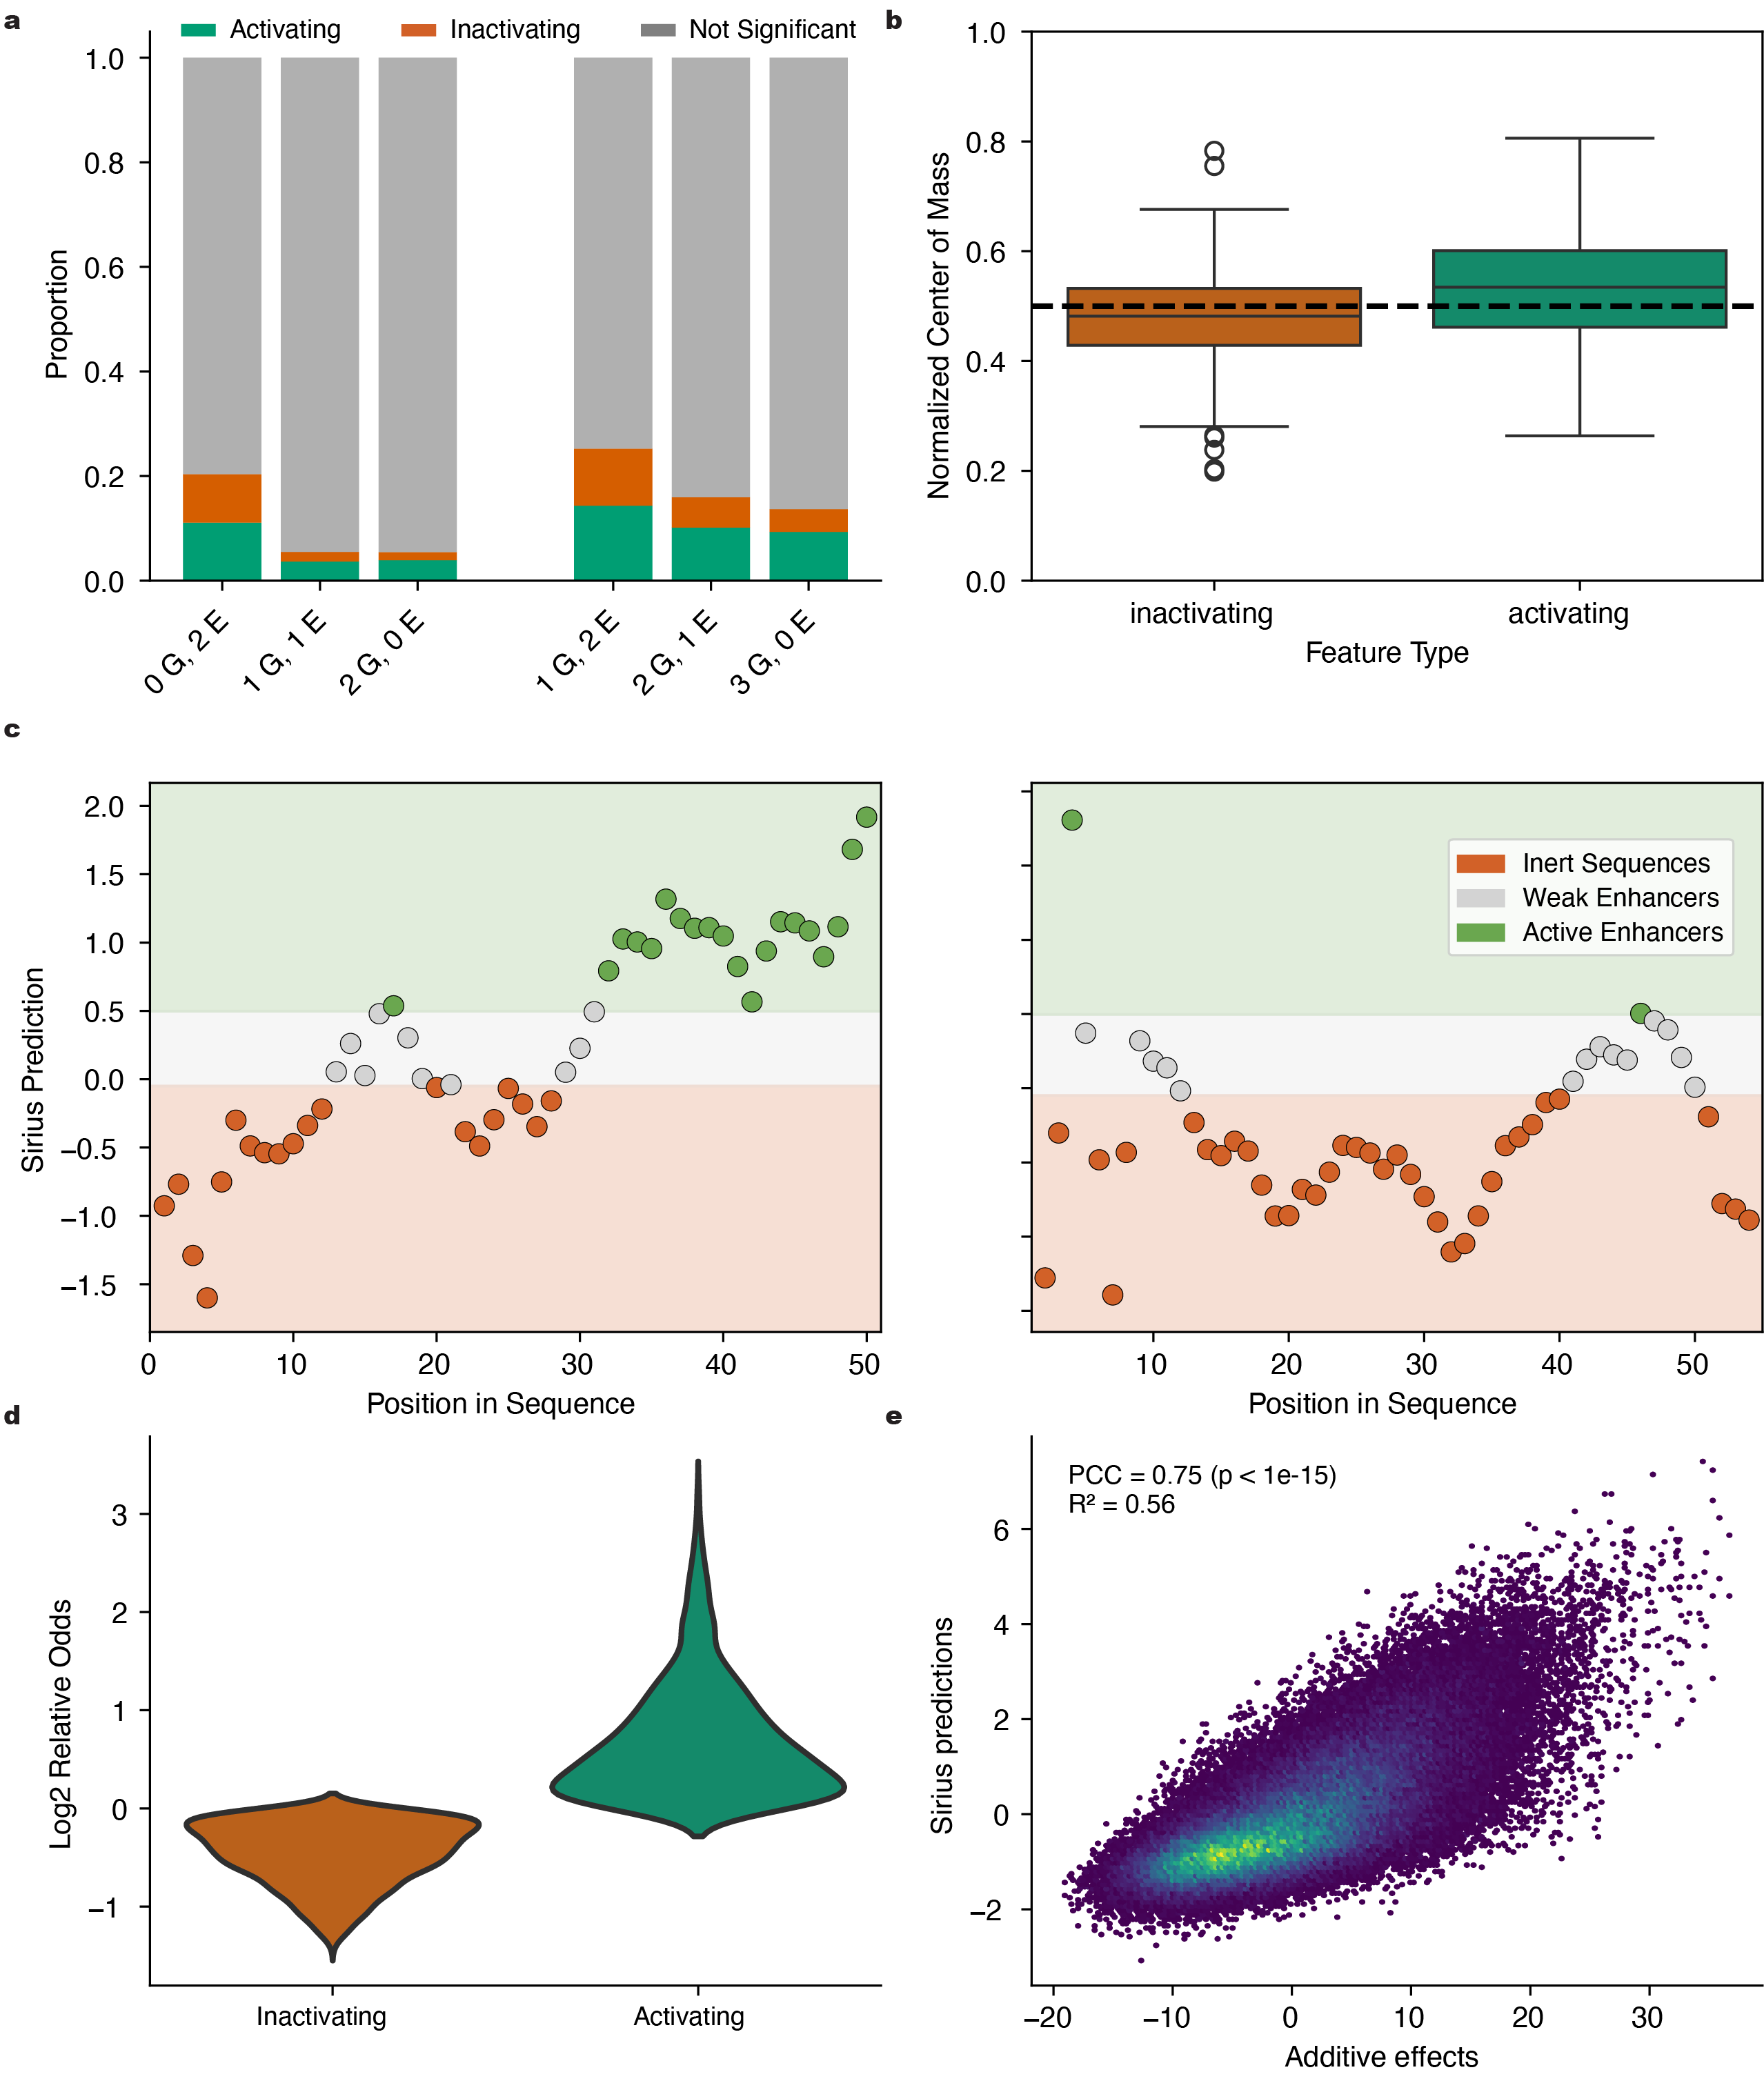
\includegraphics[width=0.85\textwidth]{2_figures-and-files/SuppFig9.png}
    \caption[Syntax feature analysis.]{\textbf{Syntax feature analysis.} \textbf{a)} Barplots of proportion of 2-site (left) and 3-site (right) syntax features split by possible combinations of ETS (E) and GATA (G) sites. P-values for Chi2 tests are 3.84e-05 and 3.06e-29 for 2-site and 3-site features respectively. \textbf{b)} Distributions for normalized center of mass of model predictions (y-axis) for inactivating and activating syntax features (see Methods). \textbf{c)} Examples of two 2-site features exhibiting periodic positional preferences. Y-axis represents Sirius predictions for syntax features across possible positions (x-axis). \textbf{Left,} g.10.E. \textbf{Right,} E.7.G. Background colors are determined by the interquartile ranges of the active enhancers and inert sequences in the OSL library. The range in between the upper quartile of the inert sequences and the lower quartile of the active enhancers is classified as weak enhancers. \textbf{d)} 2,494 single syntax changes flip a 3-site syntax feature from a negative Log2 relative mean odds (inactivating) to a positive one (activating). \textbf{e)} Scatterplot of predictions for AdditiveFeatures (x-axis) against Sirius (y-axis). Pearson correlation coefficient (PCC) and percent variance explained (R²) are annotated in the top left.}
    \label{fig:2 supplementary_9}
\end{figure}

\begin{figure}[p]
    \centering
    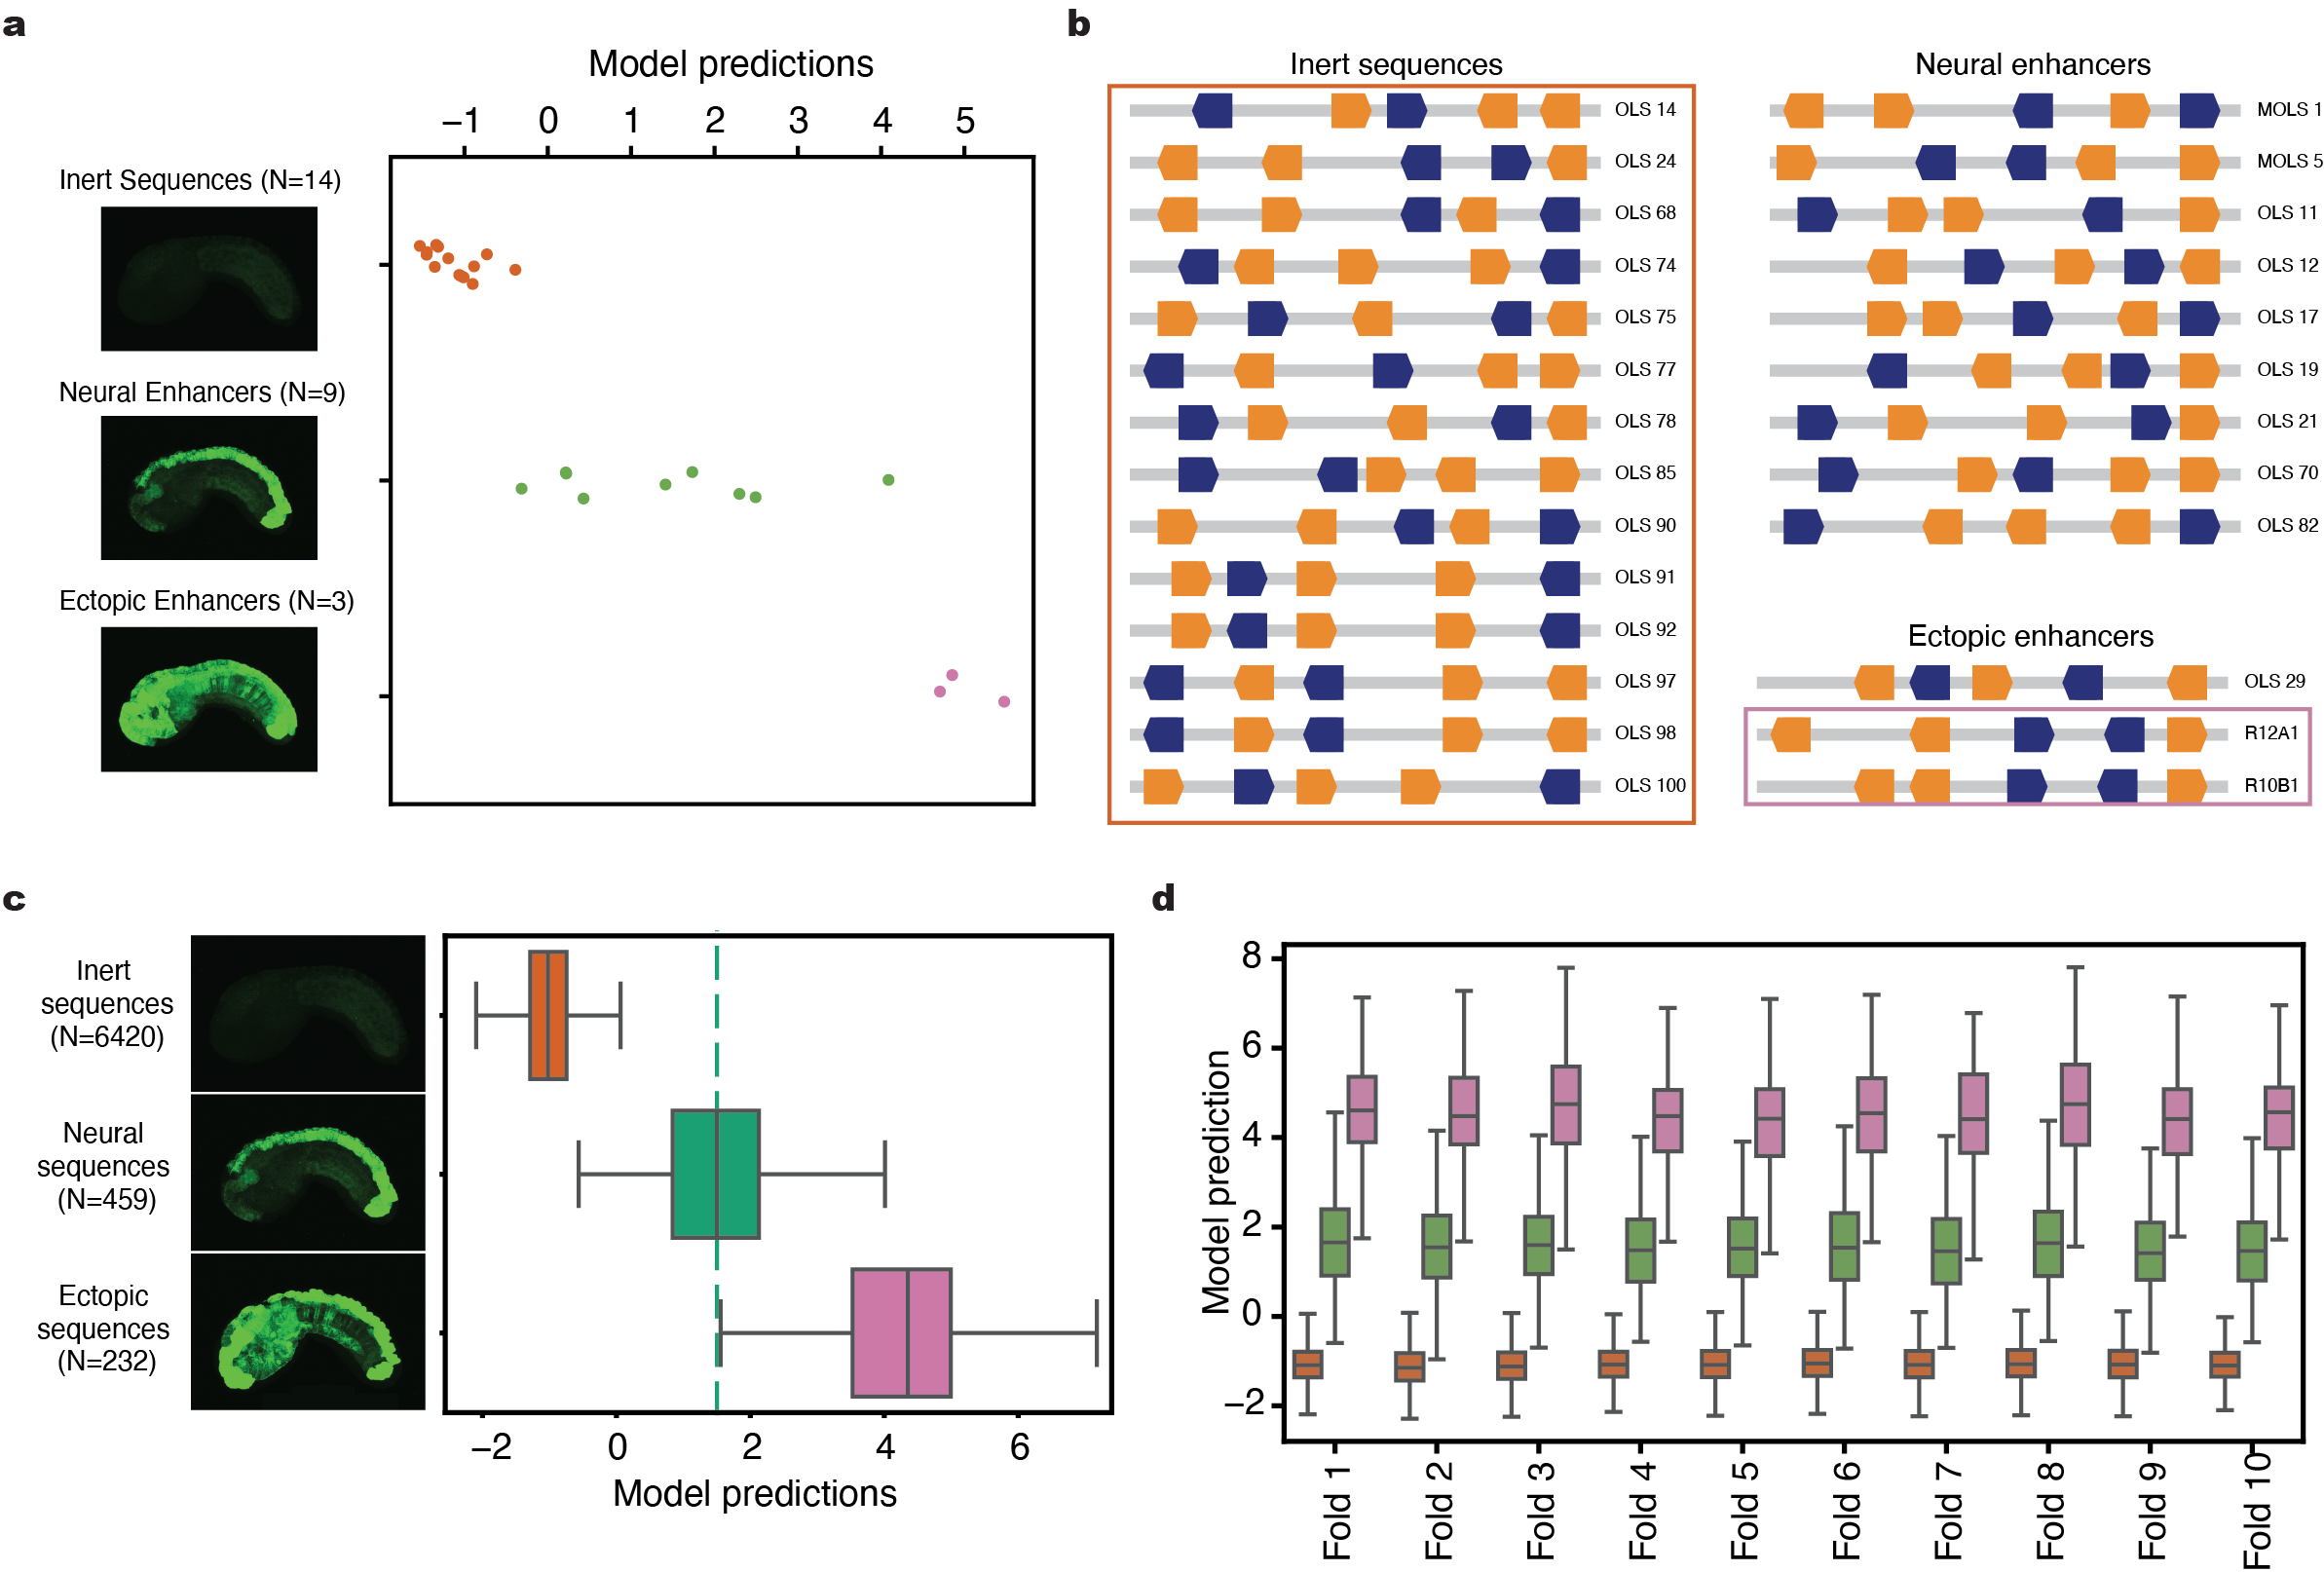
\includegraphics[width=0.9\textwidth]{2_figures-and-files/SuppFig10.png}
    \caption[Sirius predictions show implicit tissue specificity.]{\textbf{Sirius predictions show implicit tissue specificity.} \textbf{a)} Model predictions (x-axis) across validated sequences binned by tissue specificity. \textbf{b)} Syntaxes for each point in \textbf{a)} binned by tissue specificity. Colored boxes around syntaxes indicate these were used in STARS design (\textbf{Figure~\ref{fig:2 Figure 4}}). \textbf{c)} Model predictions (x-axis) across OSL sequences binned by tissue specificity (see Methods). Representative fluorescence microscopy images are shown for each bin. The green dashed line indicates the median model prediction for neural sequences targeted during STARS design (\textbf{Figure~\ref{fig:2 Figure 4}}). \textbf{d)} Model predictions (y-axis) for OSL sequences binned by tissue specificity (see Methods) for all folds of cross-validation (x-axis).}
    \label{fig:2 supplementary_10}
\end{figure}

\begin{figure}[p]
    \centering
    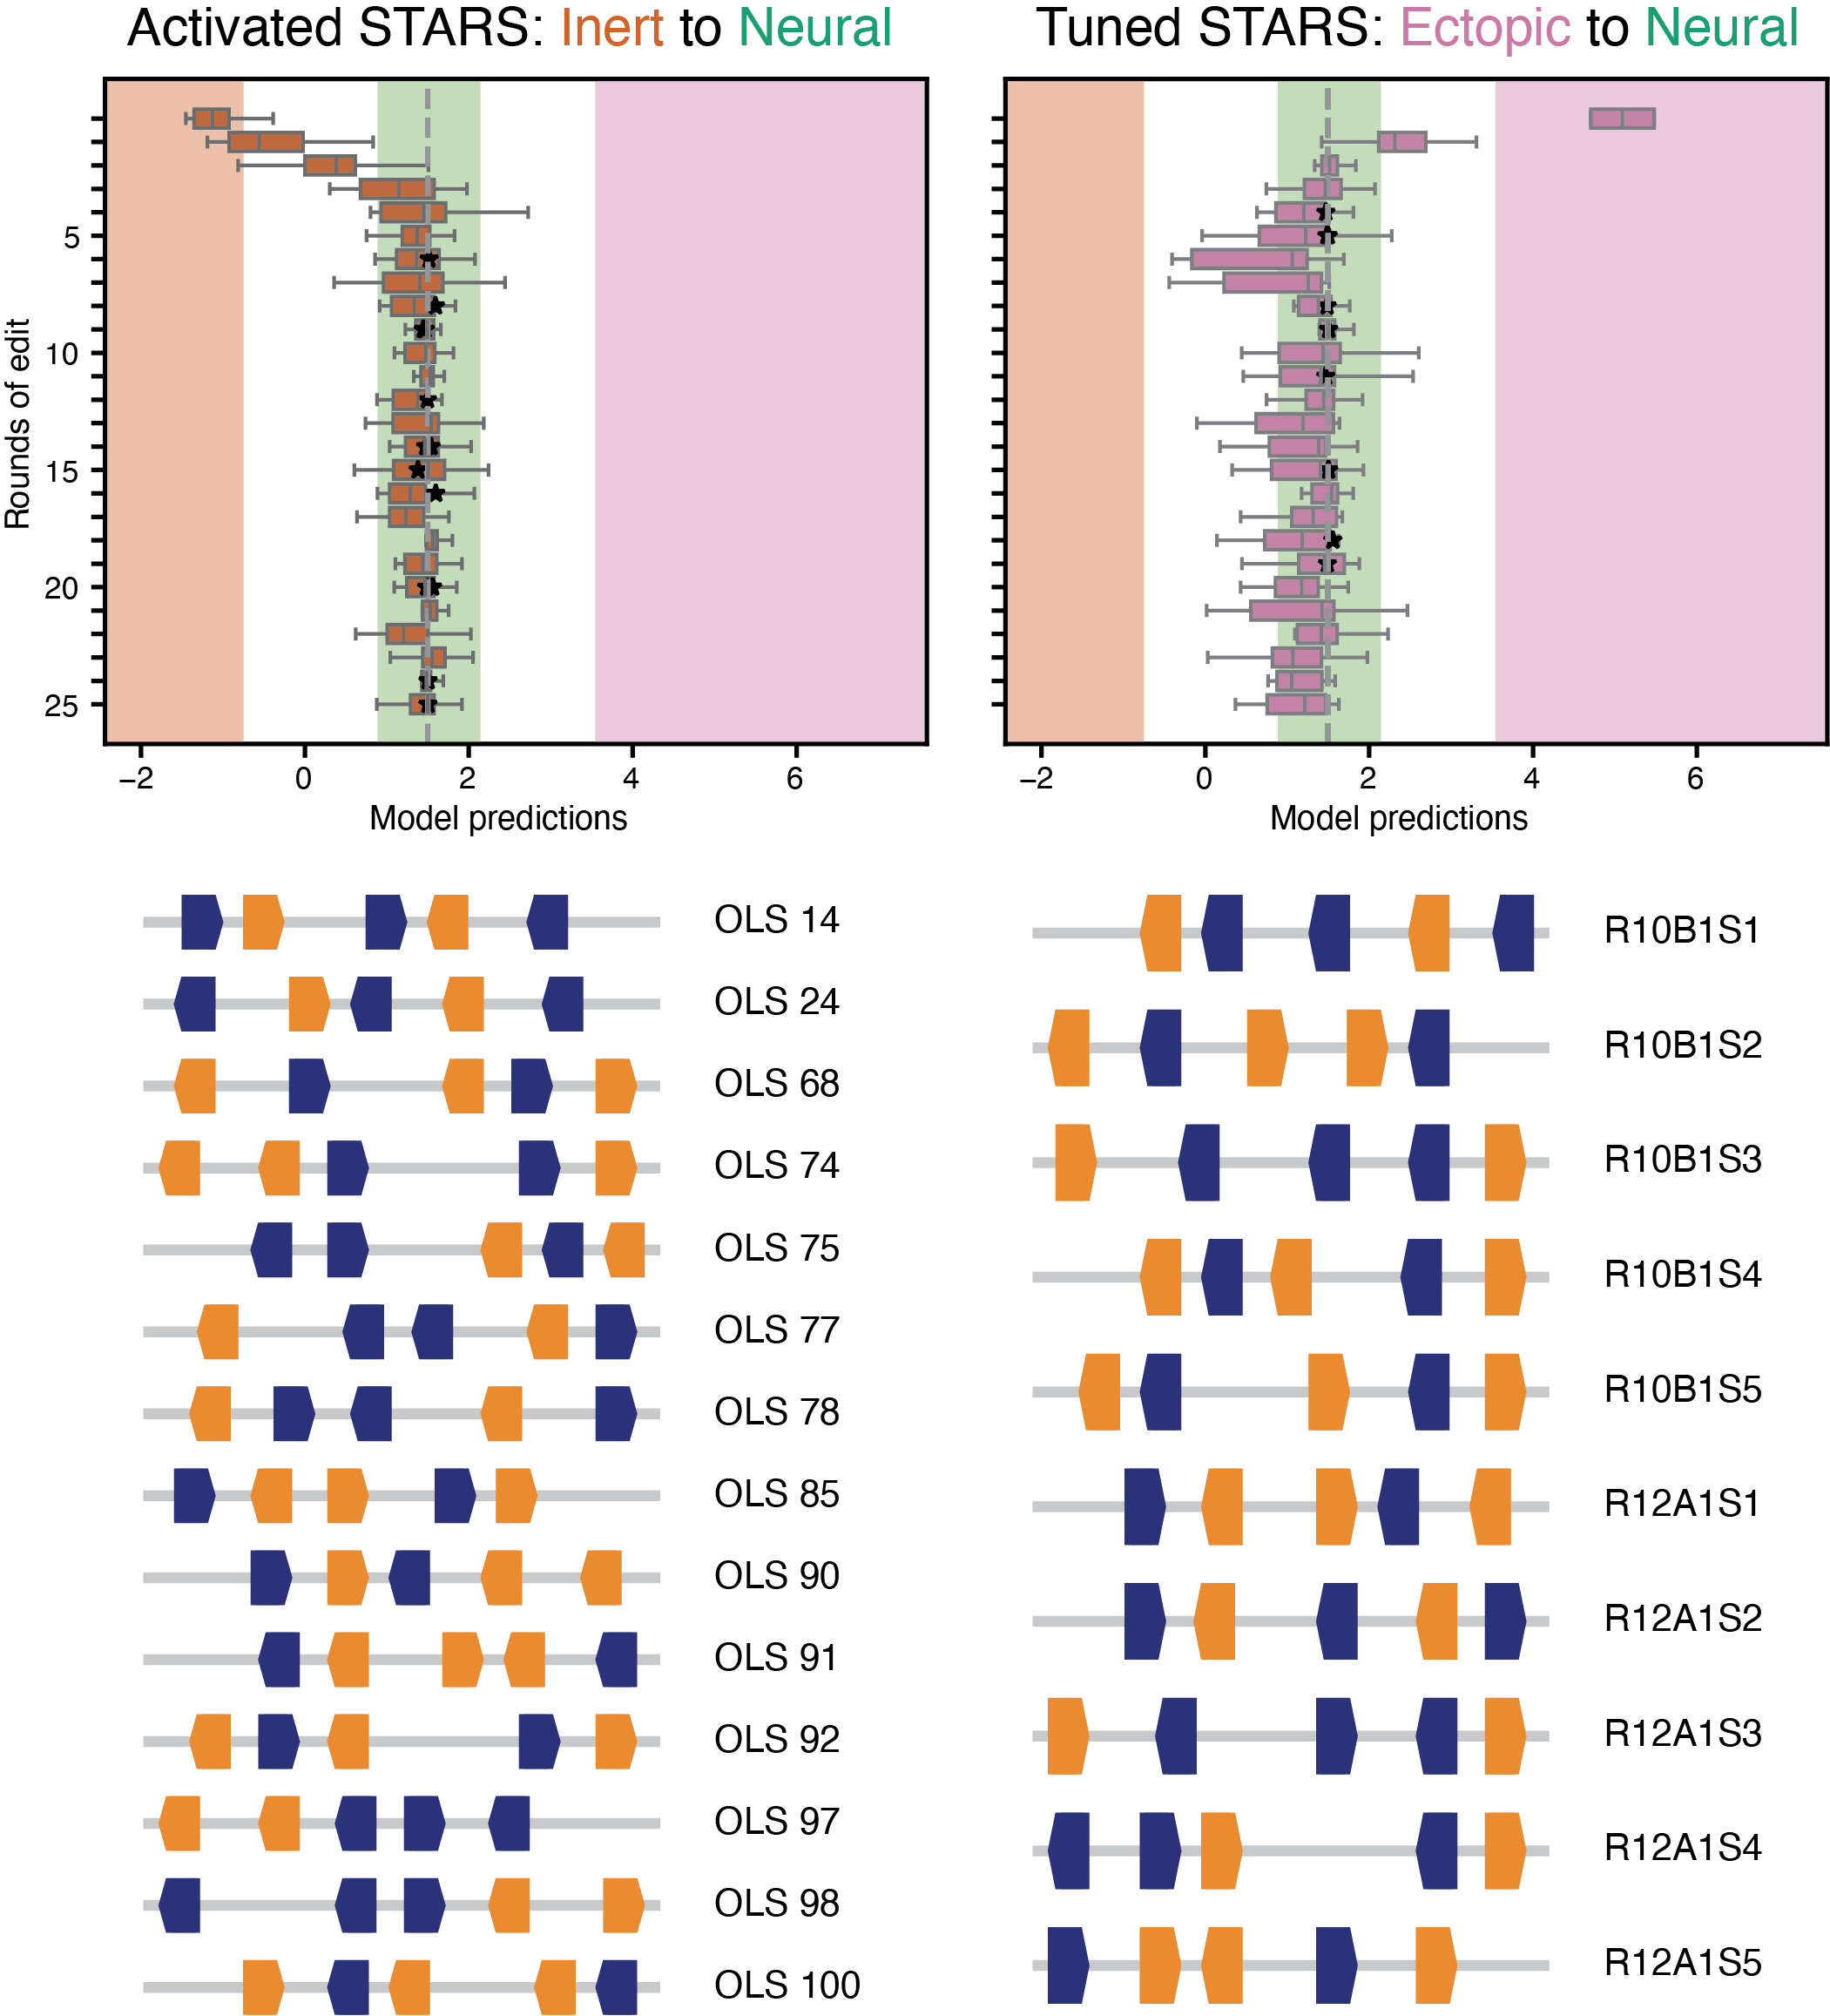
\includegraphics[width=0.88\textwidth]{2_figures-and-files/SuppFig11.png}
    \caption[24 Syntax-derived, Tissue-specific, Active, Regulatory Sequences (STARS).]{\textbf{24 Syntax-derived, Tissue-specific, Active, Regulatory Sequences (STARS).} Model prediction for each round. Background colors are determined by the interquartile ranges of the active enhancers and inert sequences in the OSL library. The range in between the upper quartile of the inert sequences and the lower quartile of the active enhancers is classified as weak enhancers. \textbf{Left,} activated STARS – syntaxes that are validated Inert Sequences are edited to activate them to a predicted Neural Enhancer syntax. \textbf{Right,} tuned STARS – syntaxes that are validated Ectopic Enhancers are edited to tune them to a predicted Neural Enhancer syntax. \textbf{Bottom,} syntax schematics for all 24 STARS. None of these syntaxes are found in the OSL library and represent novel organizations of sites.}
    \label{fig:2 supplementary_11}
\end{figure}

\begin{figure}[p]
    \centering
    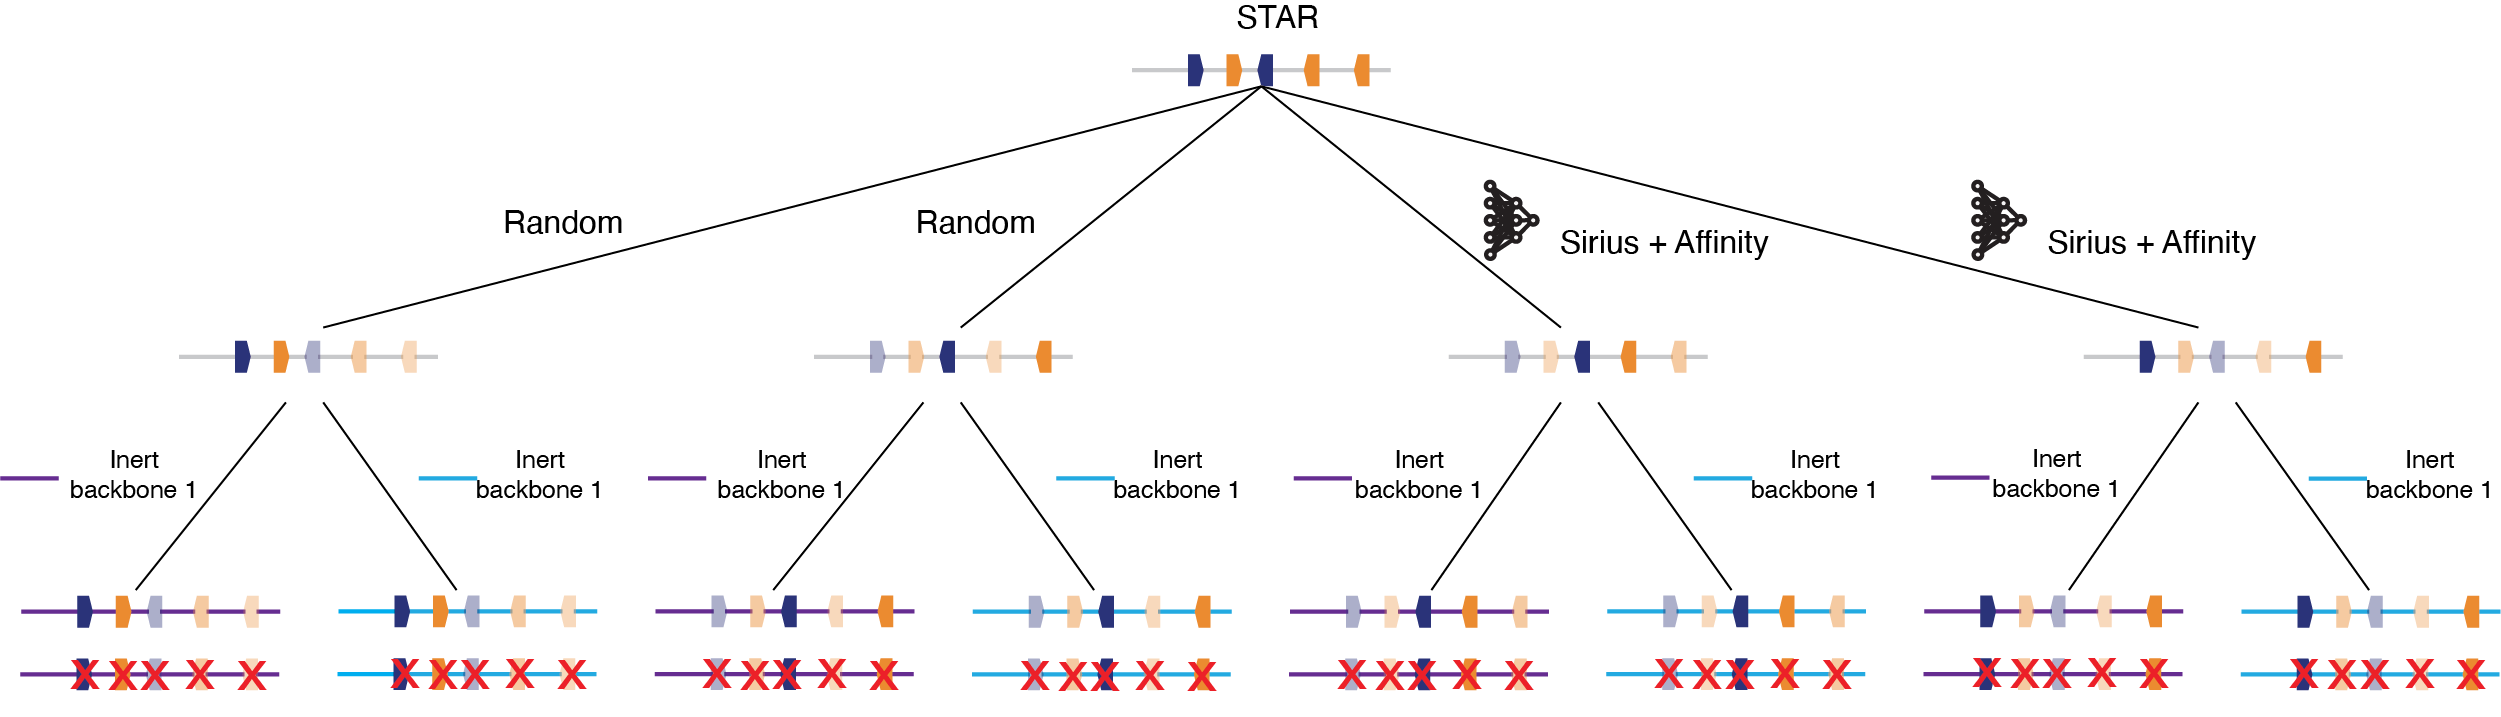
\includegraphics[width=0.88\textwidth]{2_figures-and-files/SuppFig12.png}
    \caption[STARS MPRA design.]{\textbf{STARS MPRA design.} Schematic for STARS library design and MPRA. For each of the 24 STARS, four different sets of flanking nucleotides were selected either randomly or with the Sirius + Affinity model. Two different sets of linker sequences were selected for each of the STARS from two different inert backbones. An ablated counterpart of each sequence was also synthesized where single point mutations within the core of each binding site that ablate binding of the TF are included.}
    \label{fig:2 supplementary_12}
\end{figure}

\begin{figure}[p]
    \centering
    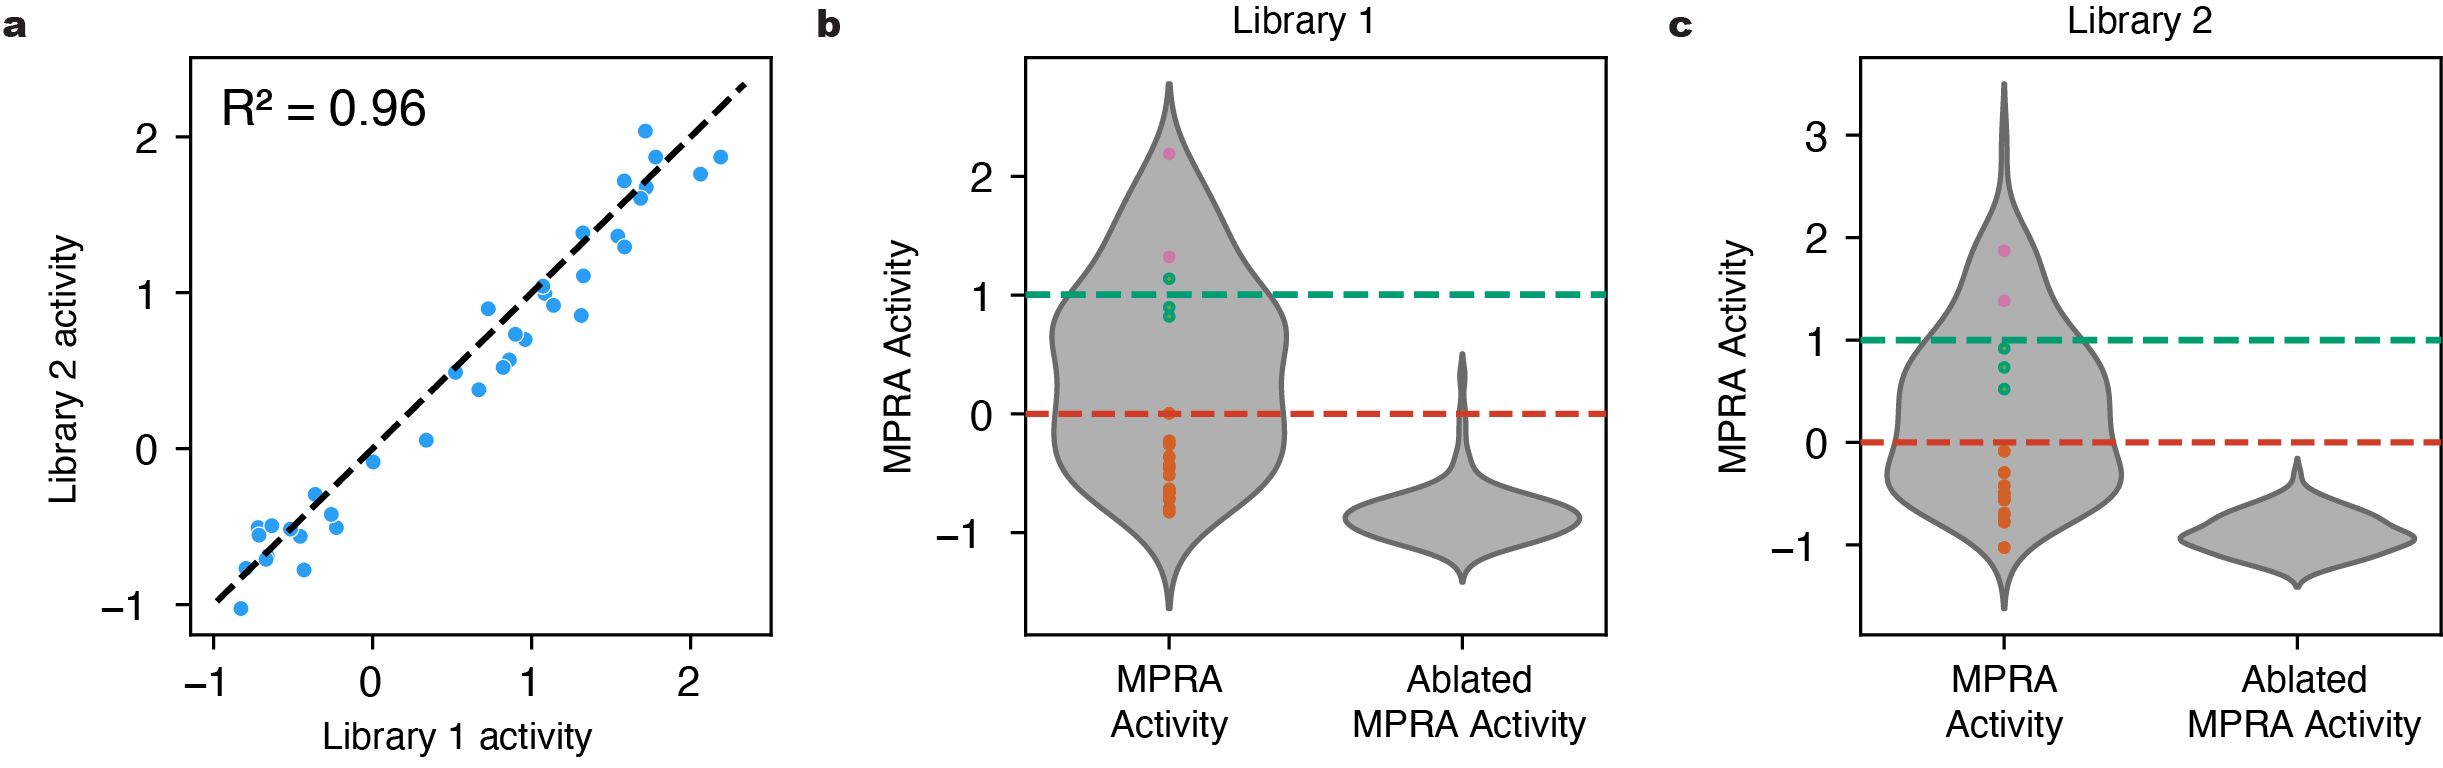
\includegraphics[width=0.88\textwidth]{2_figures-and-files/SuppFig13.png}
    \caption[Analysis of STARS MPRA.]{\textbf{Analysis of STARS MPRA.} \textbf{a)} Control reproducibility across STARS libraries. R² indicates the percentage of variance explained. \textbf{b)} Distributions of MPRA activities for library 1. \textbf{c)} Distributions of MPRA activities for library 2. The left violin for each subplot indicates the 96 WT elements tested and the right violin indicates the 96 ablated counterparts to those variants. Stripplot highlights validated controls that are inert sequences, neural enhancers and ectopic enhancers with horizontal dashed lines indicating thresholds used for classification.}
    \label{fig:2 supplementary_13}
\end{figure}

\begin{figure}[p]
    \centering
    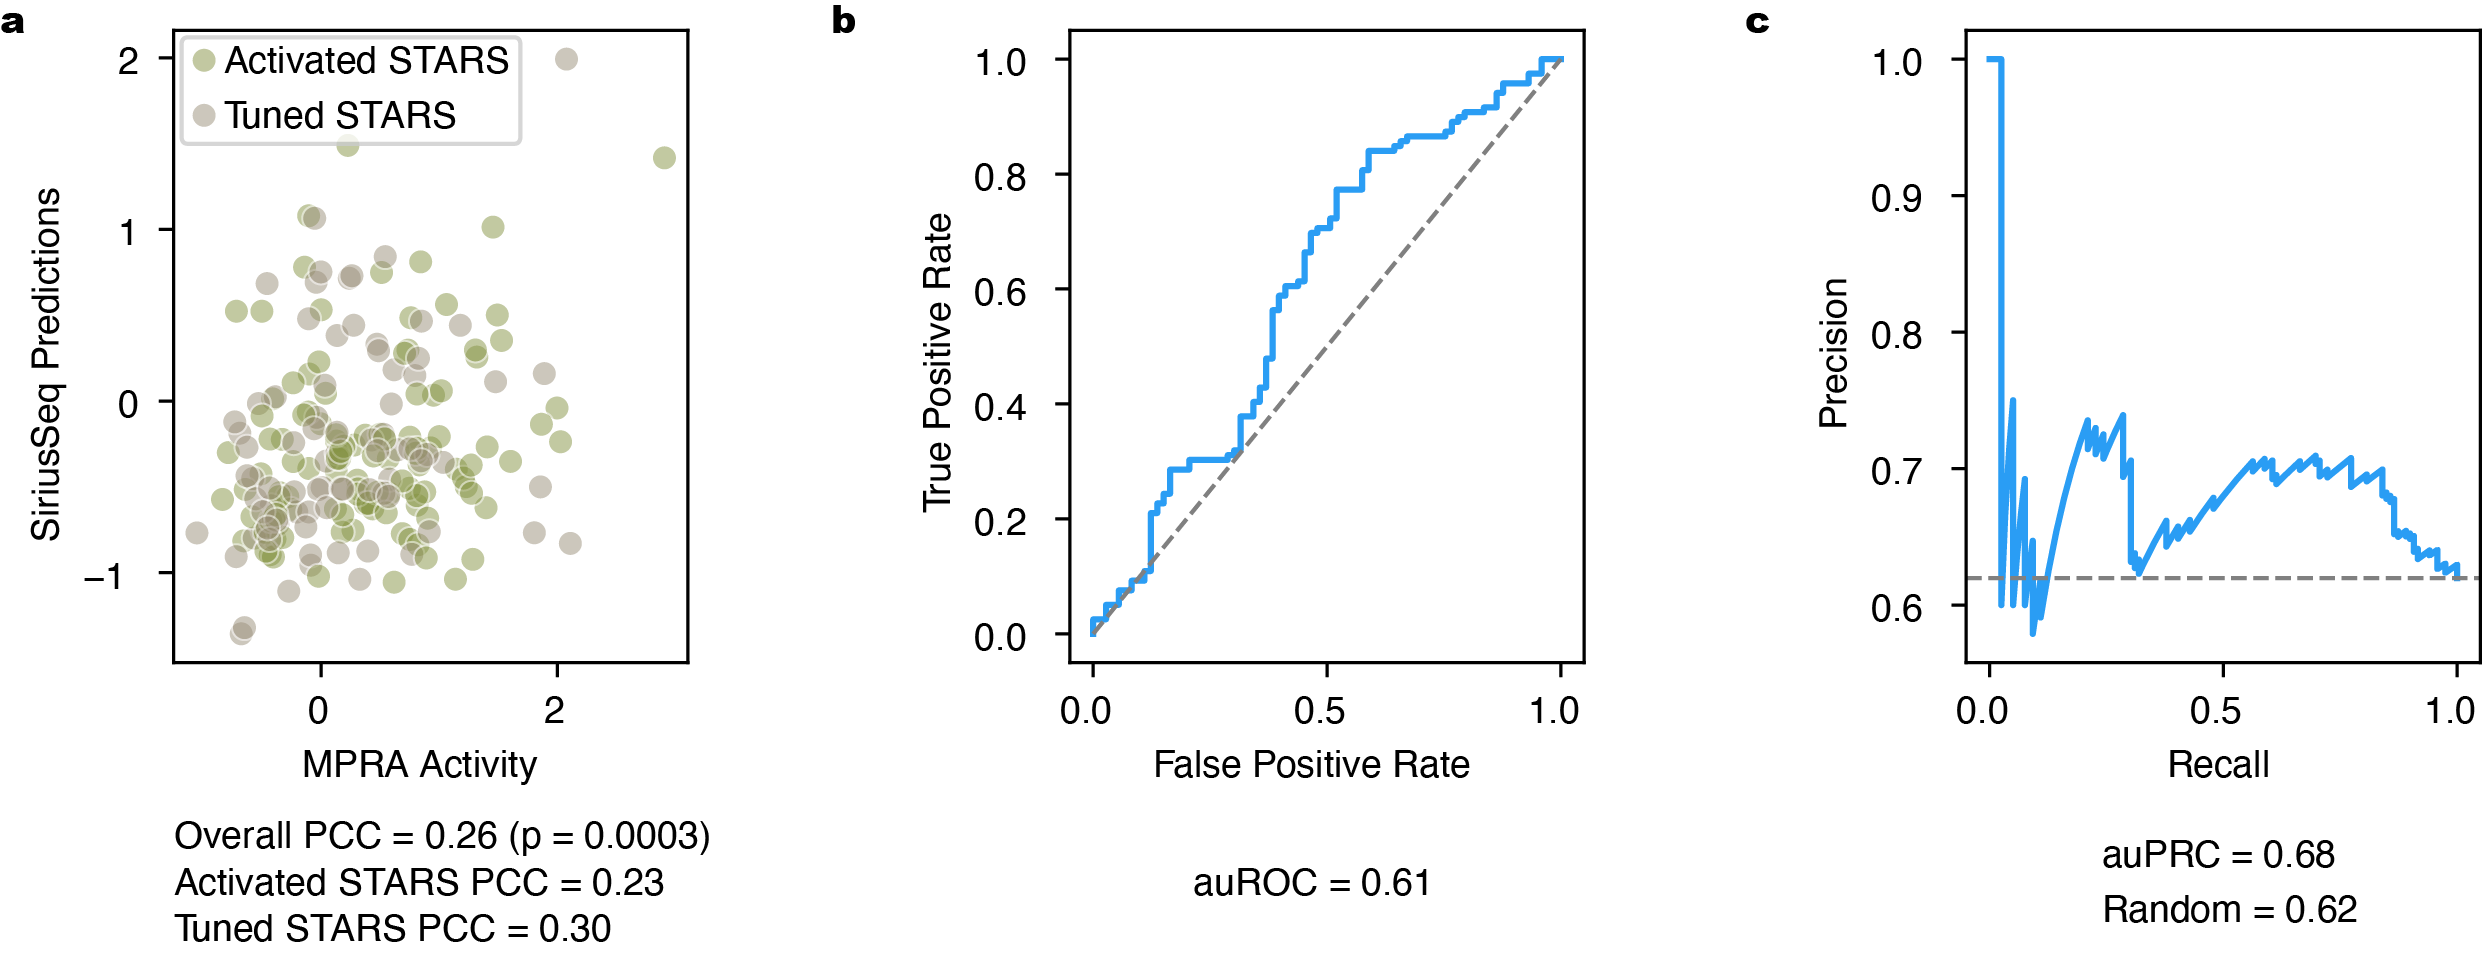
\includegraphics[width=0.88\textwidth]{2_figures-and-files/SuppFig14.png}
    \caption[SiriusSeq performance on STARS MPRA.]{\textbf{SiriusSeq performance on STARS MPRA.} \textbf{a)} Scatterplot of measured STARS MPRA activity (x-axis) against SiriusSeq predictions colored by direction of design. Pearson correlation coefficients (PCCs) for all designs and split by direction are shown below. \textbf{b)} Precision-recall and \textbf{c)} receiver operating characteristic curves for Sirius predictions on binarized activity (using controls, see \textbf{Figure~\ref{fig:2 supplementary_13}}). Area under the precision-recall curve (auPRC) and area under the receiver operating characteristic curve (auROC) are shown below the plots.}
    \label{fig:2 supplementary_14}
\end{figure}

\begin{figure}[p]
    \centering
    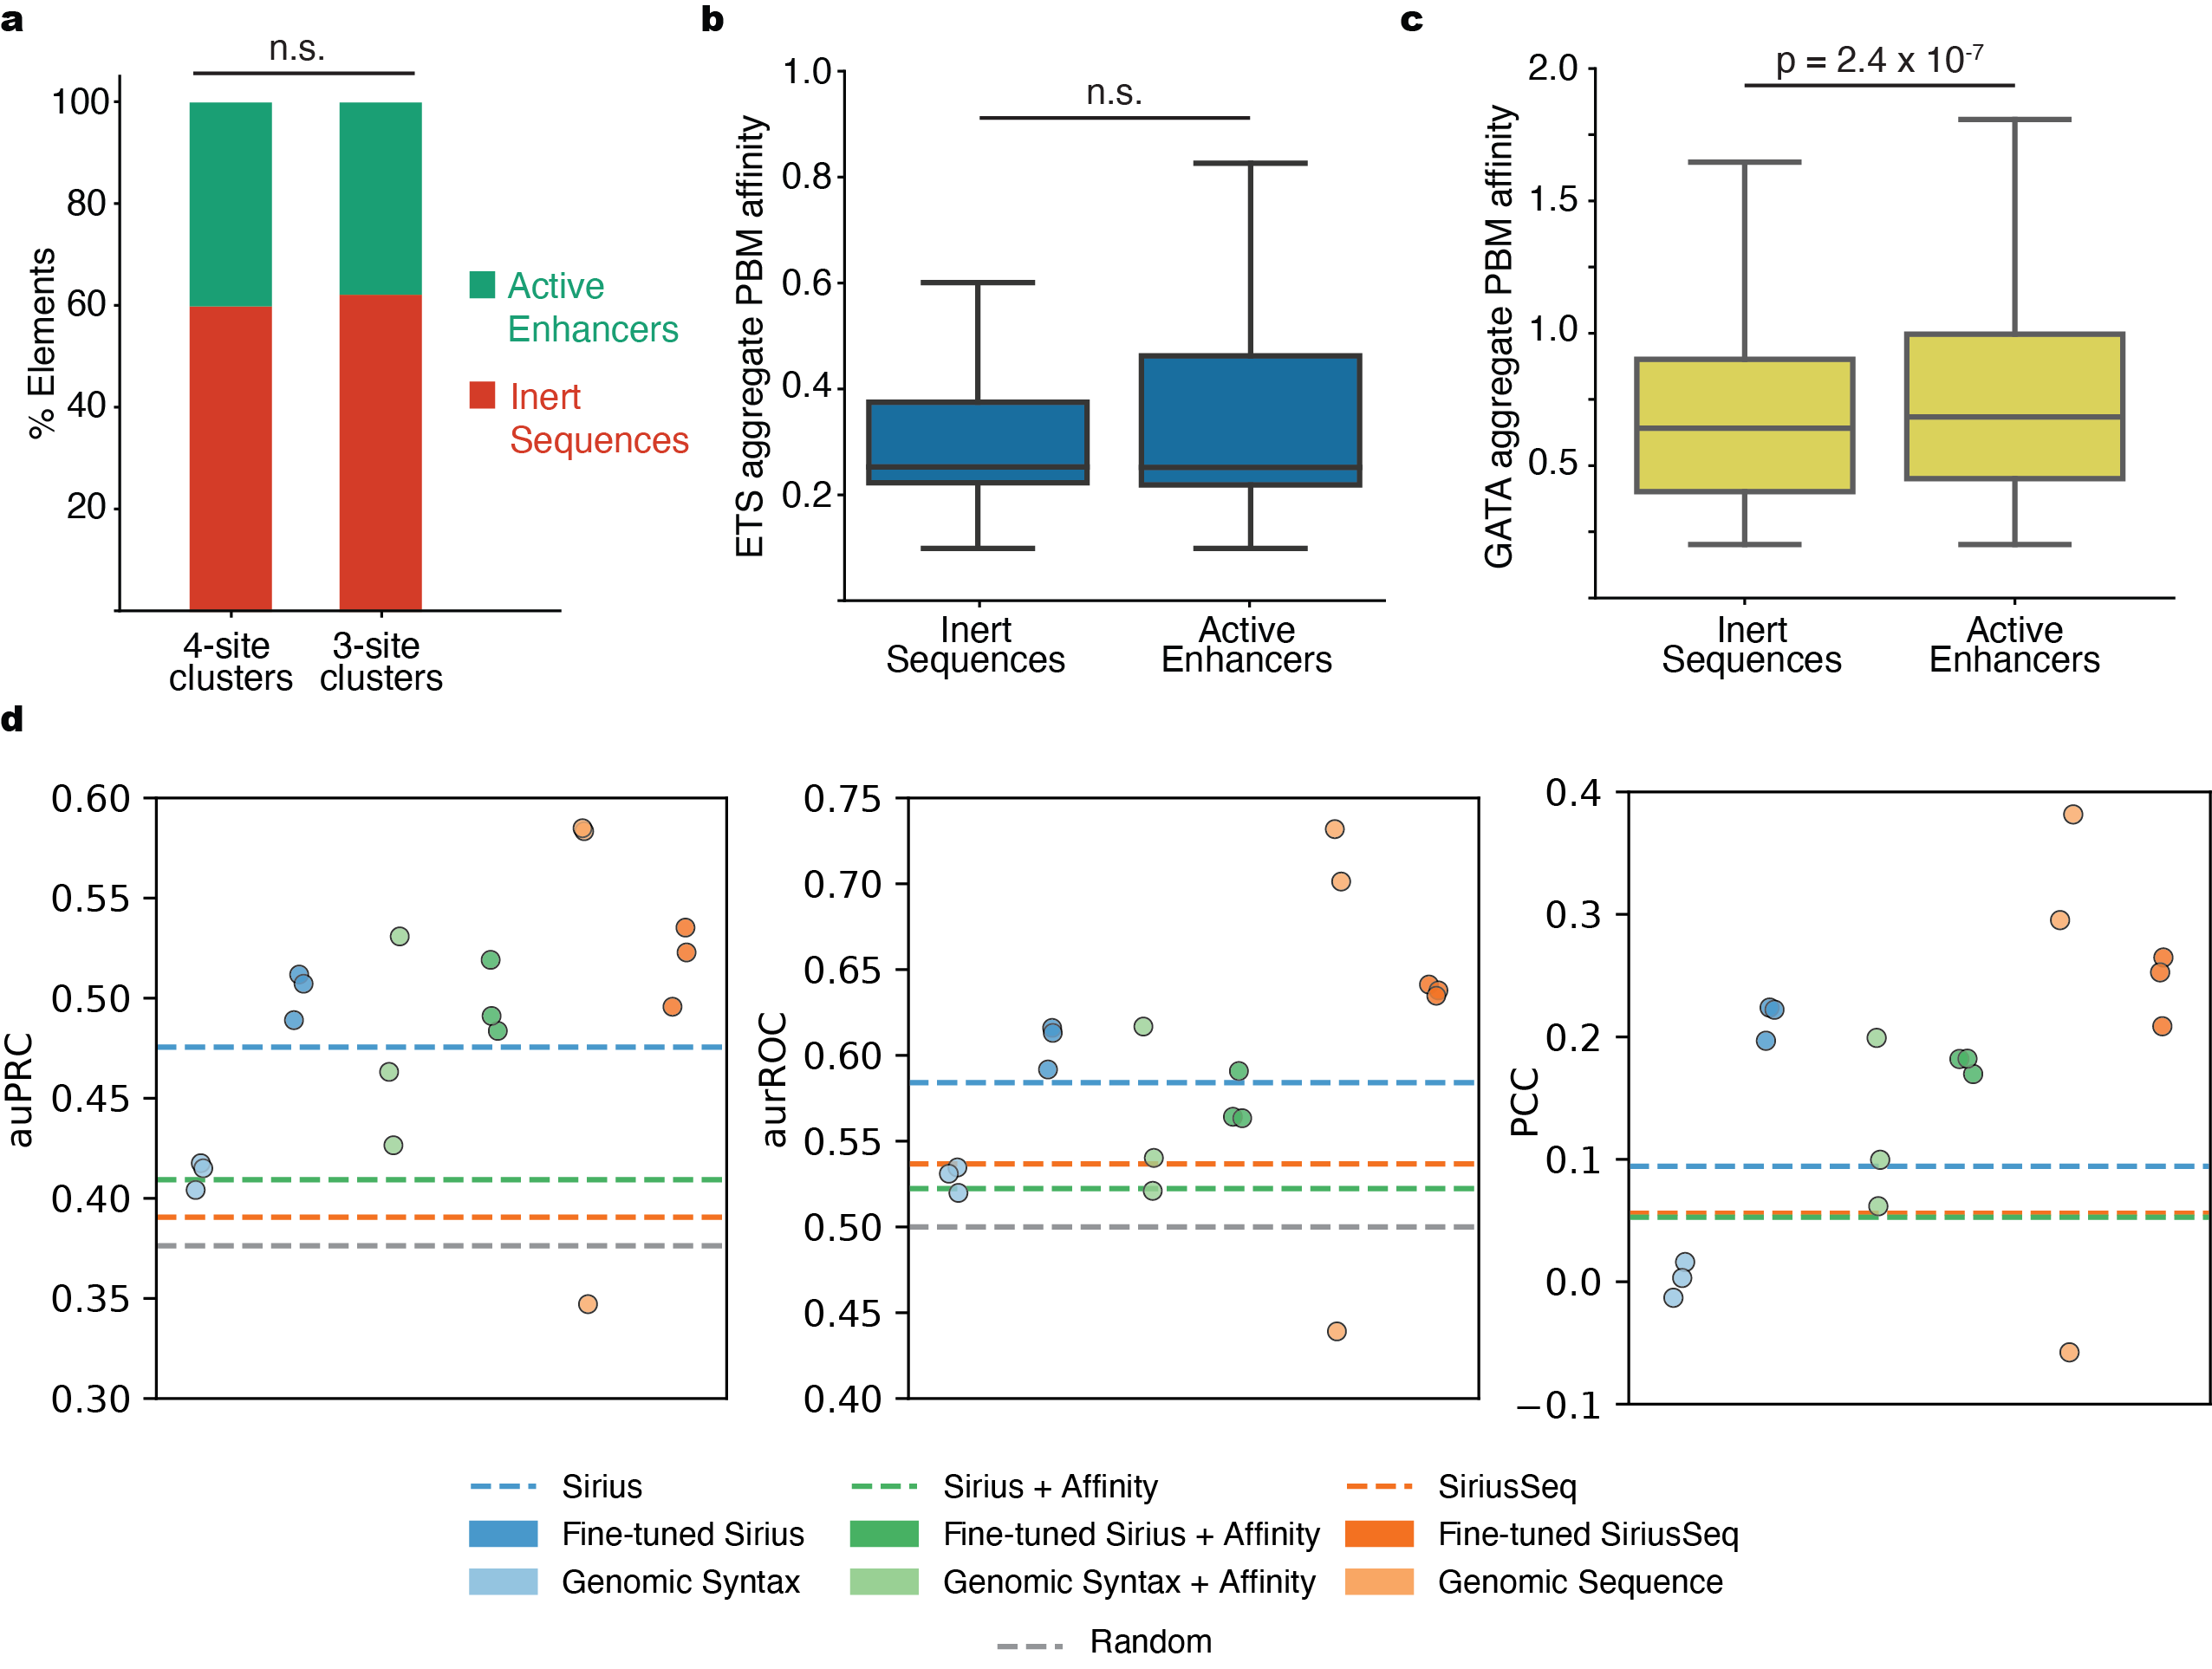
\includegraphics[width=0.88\textwidth]{2_figures-and-files/SuppFig15.png}
    \caption[Additional model training and evaluation.]{\textbf{Additional model training and evaluation.} \textbf{a)} 3-site and 4-site genomic clusters have a similar proportion of active enhancers and inert elements and are not significantly different (n.s.) by a Fisher’s exact test. \textbf{b)} Aggregate affinity of ETS and \textbf{c)} GATA across inert sequences and active enhancers within the library. The aggregate affinities are slightly increased in active elements. For GATA \textbf{c)}, this effect is significant (Mann-Whitney U test). \textbf{d)} Predictive performance on genomic cluster test set across three metrics: left, area under the precision-recall curve (auPRC); middle, area under the receiver operating characteristic curve (auROC); right, Pearson correlation coefficient (PCC). Dashed lines indicate models trained on the OSL library (single fold). All models trained on genomic library sequences were trained across three folds (i.e., each point corresponds to a fold).}
    \label{fig:2 supplementary_15}
\end{figure}

\begin{figure}[p]
    \centering
    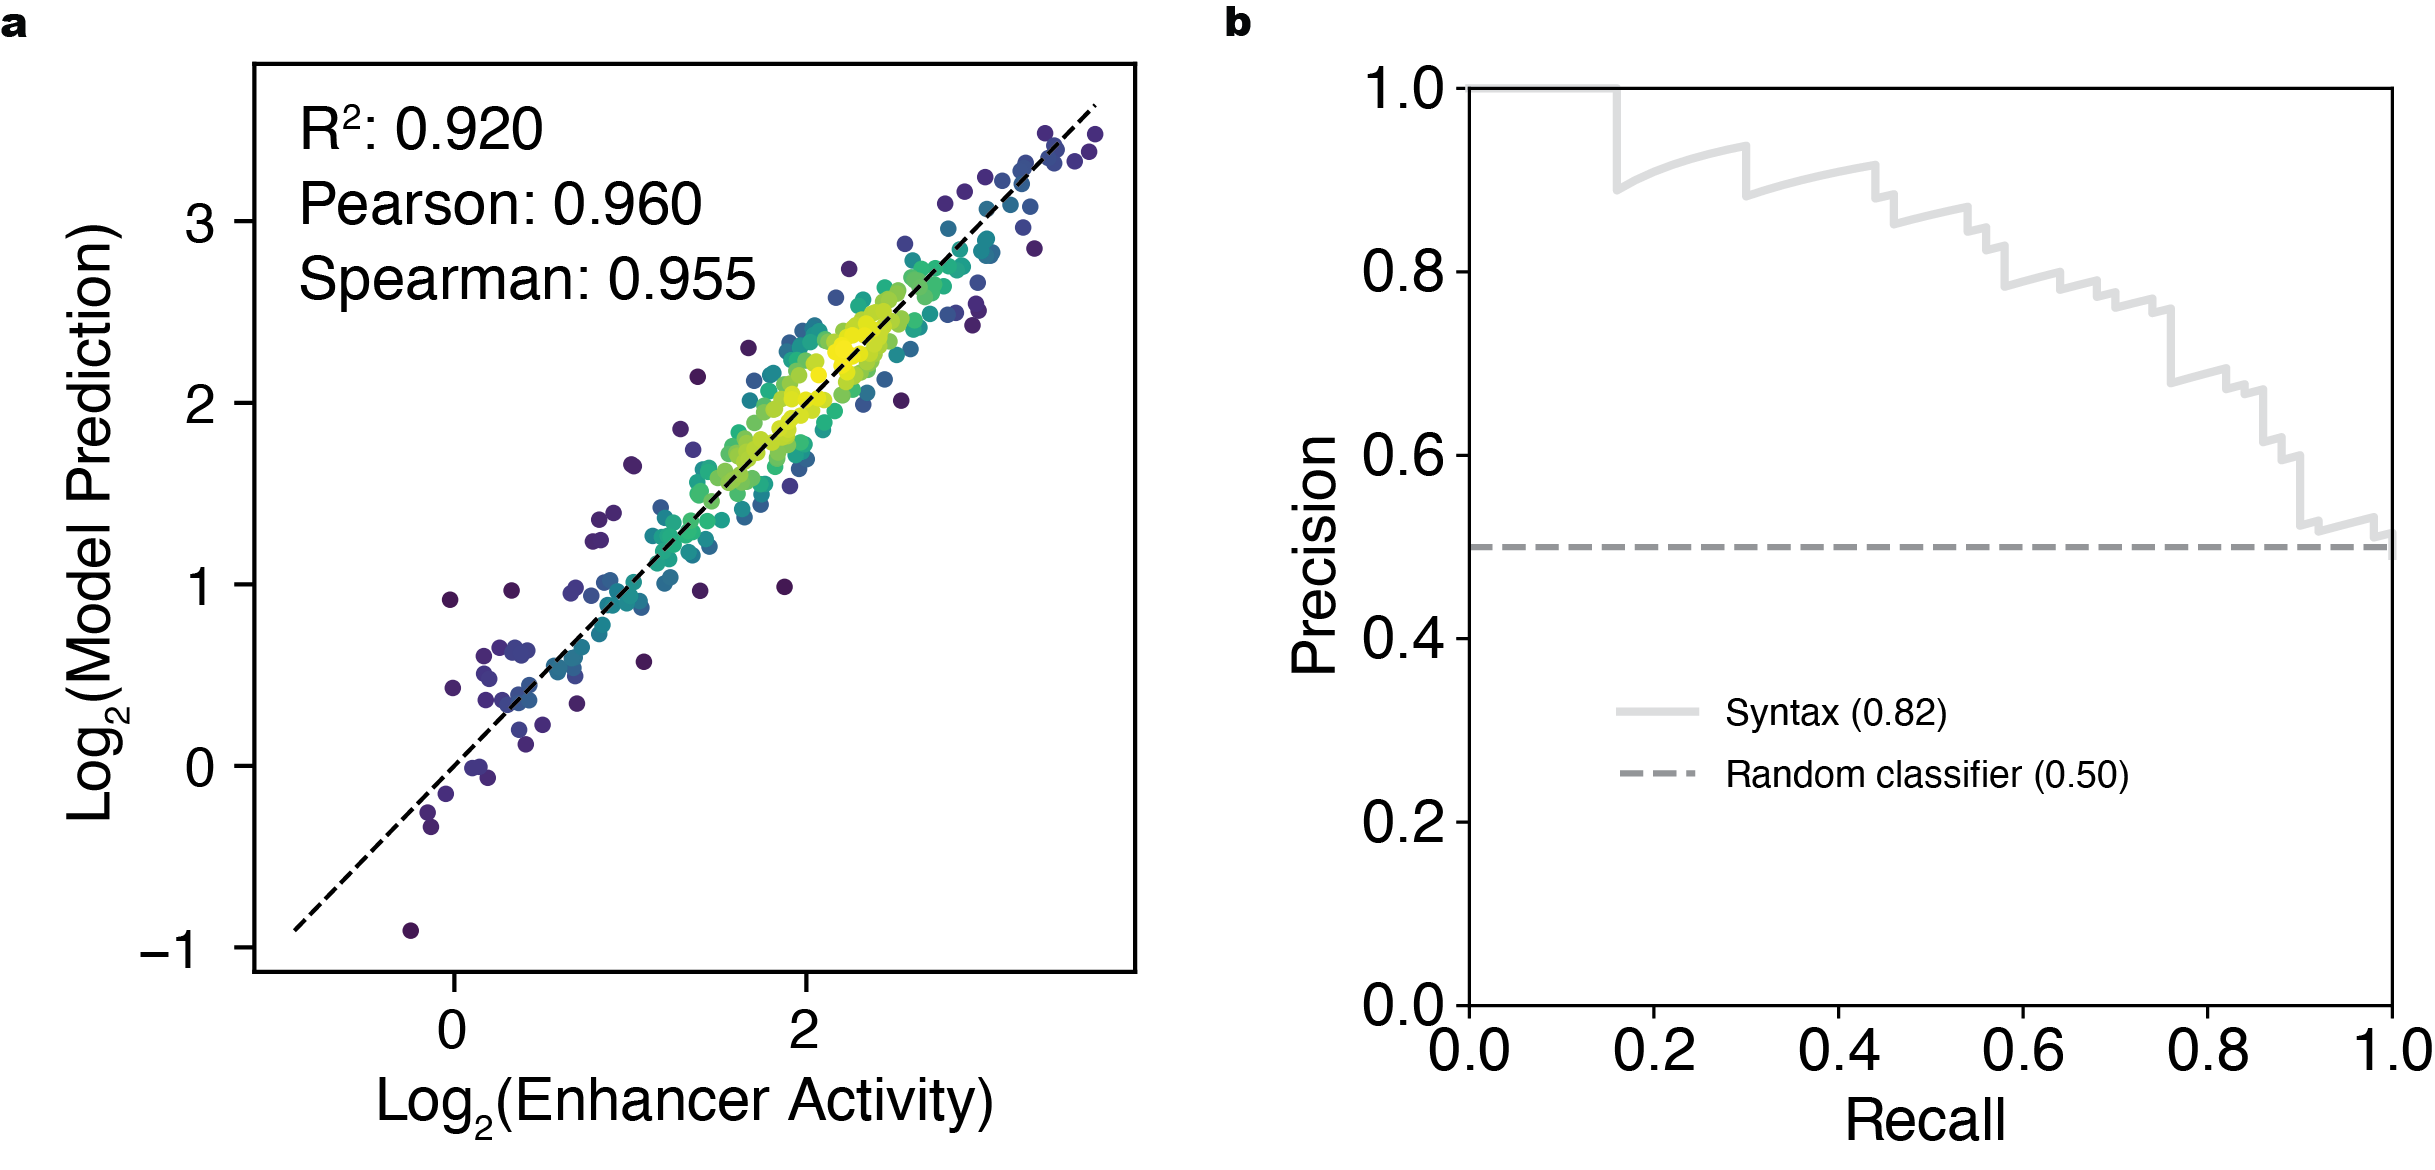
\includegraphics[width=0.88\textwidth]{2_figures-and-files/SuppFig16.png}
    \caption[Assessing the generalizability of the syntax encoding on pluripotency TF synthetic element library in mESC.]{\textbf{Assessing the generalizability of the syntax encoding on pluripotency TF synthetic element library in mESC.} \textbf{a)} Scatterplot of enhancer activity (x-axis) vs model predictions (y-axis) for model trained on synthetic library of four pluripotency transcription factors in mouse embryonic stem cells (mESCs). Percentage of variance explained (R²), Pearson correlation coefficient (PCC) and Spearman’s $rho$ are annotated. \textbf{b)} Precision-recall curve for syntax + affinity model trained on genomic sequence library in mESCs. Areas under the precision-recall curve (auPRC) are indicated in parentheses.}
    \label{fig:2 supplementary_16}
\end{figure}
